\documentclass[9pt]{beamer}
\usepackage{graphicx}
\graphicspath{{Images/}}
\usepackage{media9}
\addmediapath{Videos/}
\usepackage{caption}
\usepackage{multicol}
\usepackage{media9}
\usepackage{xcolor,colortbl}
%\definecolor{green}{rgb}{0.1,0.1,0.1}
\newcommand{\done}{\cellcolor{green}}  %{0.9}
\newcommand{\hcyan}[1]{{\color{green} #1}}
\usepackage{amsmath}
\mode<presentation> {
\usetheme{Warsaw}
}

\usepackage{graphicx} % Allows including images
\usepackage{booktabs} %

\title[Statistical Model for Improved Surface Detection]{A Statistical Model for Improved Surface Detection} % The short title appears at the bottom of every slide, the full title is only on the title page

\author{Samuel Smith} % Your name
\institute[Birmingham City University] % Your institution as it will appear on the bottom of every slide, may be shorthand to save space
{
Birmingham City University \\ % Your institution for the title page
\medskip
\textit{samuel.smith@mail.bcu.ac.uk} % Your email address
}
\date{\today} % Date, can be changed to a custom date

\begin{document}

	\begin{frame}
		\titlepage % Print the title page as the first slide
	\end{frame}



	\begin{frame}[shrink]
		\frametitle{Overview} % Table of contents slide, comment this block out to remove it
\begin{multicols}{2}
\tableofcontents
\end{multicols}
\end{frame}
	

%------------------------------------------------
\section{Problem Definition}
\subsection{Rationale}
	\begin{frame}
		\frametitle{Rationale}

			\begin{itemize}
				\item Three dimensional image data is becoming the common modality for many non-destructive testing, image analysis, visualisation and biomedical imaging systems. Typically:
				\begin{itemize}
				
				\item Computed Tomography
				\item Magnetic Resonance Imaging / functional MRI
				
				\end{itemize}
				
					\item These high level processes require low level image processing techniques.
				\item Improvements offered in low level techniques, should offer improvements to higher level applications.
			\end{itemize}
	
	\end{frame}
%------------------------------------------------



\subsection{Surfaces} 
\begin{frame}[shrink]
\frametitle{Three Dimensional Data}
\begin{figure}
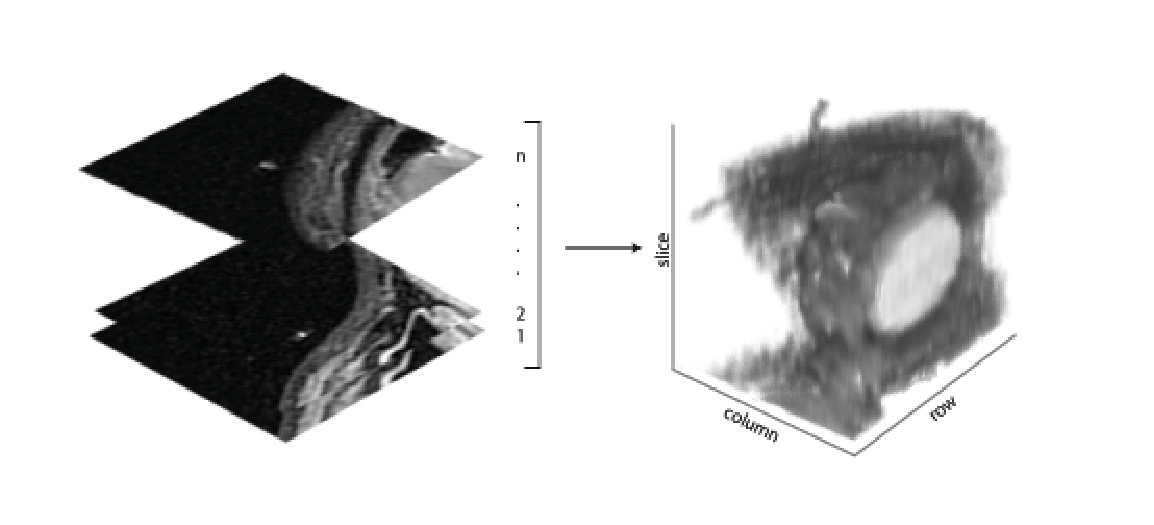
\includegraphics[scale=0.5]{slices.eps}
\end{figure}

Three dimensional image data is stored as 3 dimensional array, consisting of a stack of two dimensional slices.
\end{frame}

	\begin{frame}
			\frametitle{What is a Surface?}
				
				\begin{itemize}
						\item A surface is an interface which exists in 2 or 3 dimensional data, it describes boundary, or plane, which separates two or more different regions.\\
						\item This boundary could be between two or more areas of different:
				
						\begin{itemize}
								\item Voxel Intensities
								\item Colour
								\item Texture

						\end{itemize}
				
				\end{itemize}

	\end{frame}
%------------------------------------------------	
	\begin{frame}
			\frametitle{What is a Surface?}


				\begin{figure}
				\begin{tabular}{c c}
	
						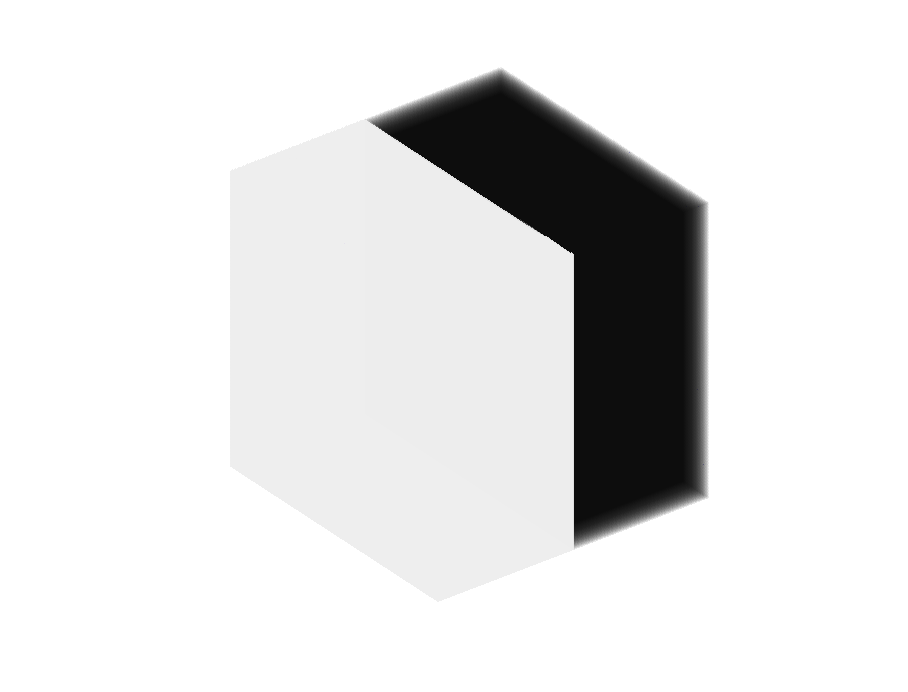
\includegraphics[scale=0.2]{intensity3d} &

						
\includegraphics[scale=0.2]{colourinterface3d}\\
						a & b\\
		
						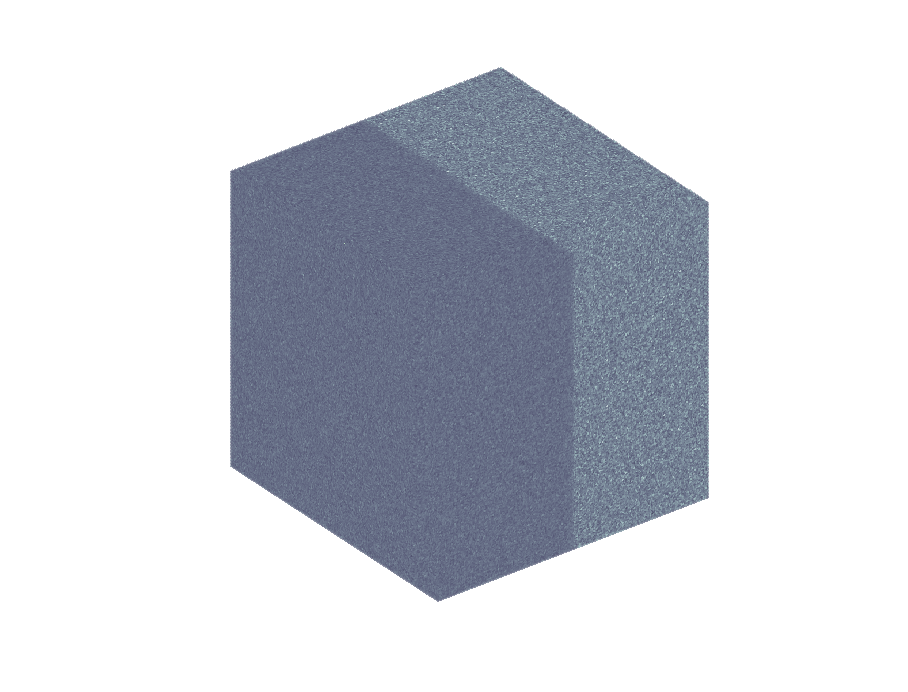
\includegraphics[scale=0.2]{statinterface} &
	
						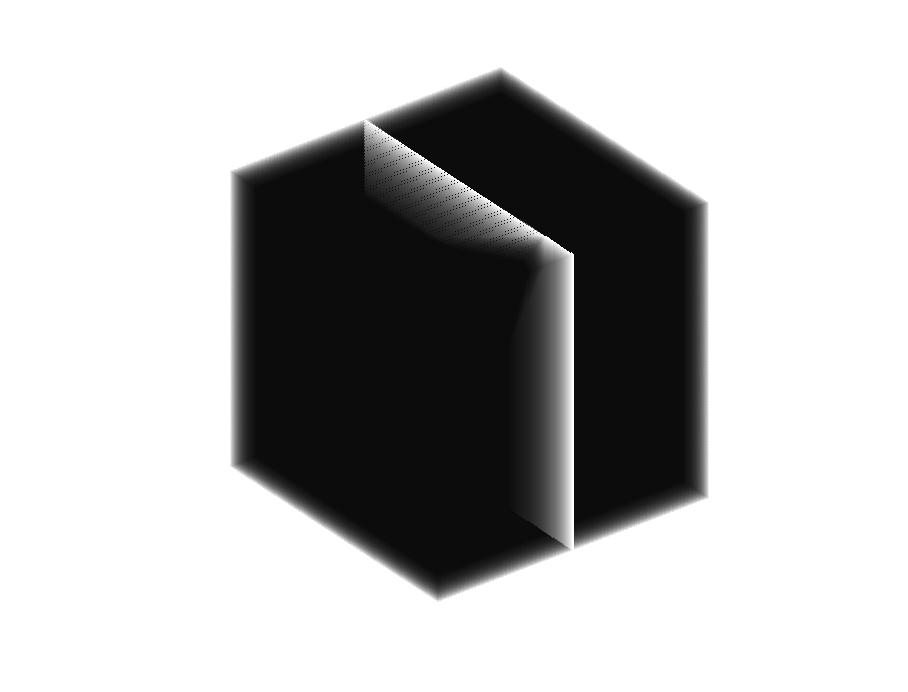
\includegraphics[scale=0.2]{edge3d2}\\
						c & d
							
				\end{tabular}
						
						\caption{ a) Intensity Interface. b) Colour Interface. c) Texture Interface. d) Interface Location}
				\end{figure}
	
	\end{frame}
%---------------------
	\subsection{Problems}
	
		\begin{frame}
				\frametitle{3D Surfaces}

						\begin{itemize}
							\item Optimal plane of application is not known a priori
								\item Surfaces which lie in the plane of edge detection are not detected. Instead an outer edge of the surface is identified
						\end{itemize}
				
	\begin{flushright}
				\begin{figure}
								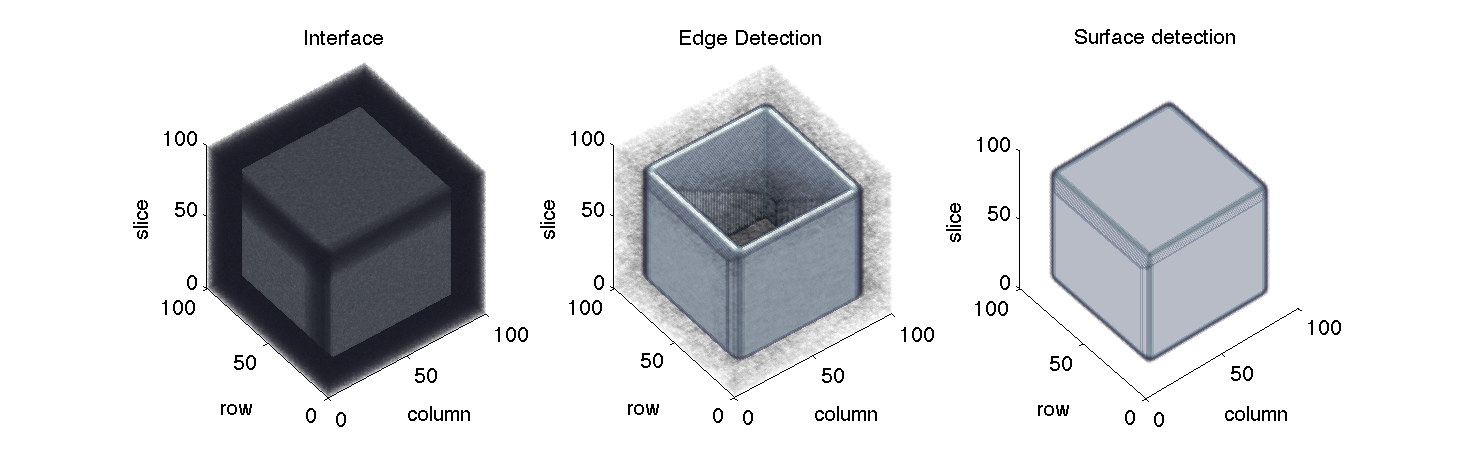
\includegraphics[scale=0.45]{fail2d}
					\end{figure}
	\end{flushright}

			\end{frame}
			
			\begin{frame}
\frametitle{3D Surfaces}
						\begin{itemize}
							\item Optimal plane of application is not known a priori
								\item Surfaces which lie in the plane of edge detection are not detected. Instead an outer edge of the surface is identified
						\end{itemize}
\begin{center}
			\includemedia[activate=onclick, width=0.75\textwidth]{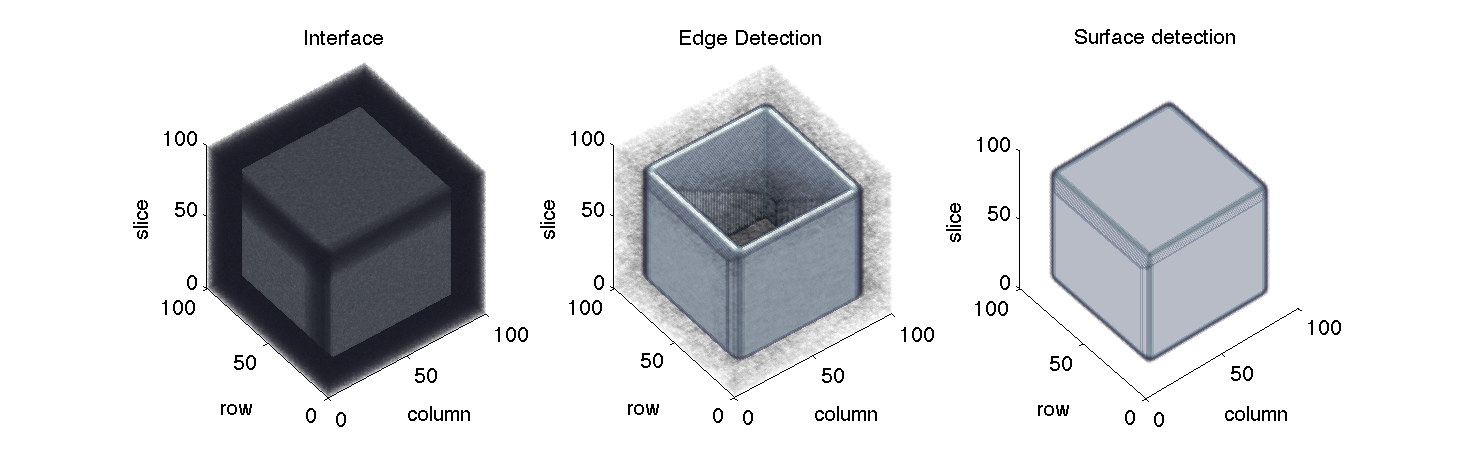
\includegraphics{fail2d}}{cubes1.mp4}
\end{center}
\end{frame}

\section{3D surface detection methods}

\begin{frame}
\frametitle{ Criteria for edge/surface detection }
When designing a surface detection filter, there are certain criteria that needs to be met. Canny defined the following criteria for edges, but the following holds true for surfaces.
\begin{itemize}
\item Criterion 1: Good detection.\\
Minimising the number of number of missed surface points, as well as minimising the number of spurious responses.
\item Criterion 2: Good localisation.\\
The points marked as surface points by the operator should be as close as possible to the center of the true surface.
\item Criterion 3: Single Response.\\
There should be only one response to a single surface. Duplicate responses for surfaces should be eliminated.
\end{itemize}
\end{frame}
\begin{frame}
\frametitle{ Methods of Surface Detection}
Methods for segmenting surface information from 3D image datasets.
\begin{itemize}
\item Gradient Based Operators.
\item Steerable filters.
\item Statistical Surface Detection.
\end{itemize}
\end{frame}
\subsection{Gradient}
\begin{frame}
\frametitle{Gradient based methods}
Gradient methods can be broadly described as methods which use convolution to approximate the first and second derivative of images with regard to their intensity values. Where sharp changes in pixel intensities exist, these positions usually correspond to the location of a boundary.
\begin{itemize}
\item Sobel.\\
An efficient convolution based method for determining the first derivative of an image.
\item Laplacian. \\
Takes the second derivative of an image.
\item Canny.\\
Applies Gaussian smoothing, non maximum suppression and hysteresis thresholding. Giving improved response in noisy images, and produces a single response for a single interface. For a long time considered the optimal method.
\end{itemize}
\end{frame}
\subsection{Steerable}
\begin{frame}
\frametitle {Steerable Filter}
\begin{itemize}

\item State of the art method for surface detection.
\item Developed by Aguet et al, extending upon the work of Jacob and Unser.
\item The design of the filters are based on ``Canny-like criteria", giving an optimal response for curves, edges and surfaces, while suppressing noise and unwanted image texture.
\item This method utilises the concept of oriented filter masks to determine the maximum response in surface detection, and adaptive filtering.
\end{itemize}
\end{frame}
\begin{frame}[shrink]
\frametitle{ 2D Statistical Edge Detection}
\begin{multicols}{2}
\begin{itemize}
\item Pixel intensity values are extracted using a simple 2D neighbourhood mask. 
\item The mask is divided into two sample regions, to which a statistical test is applied measuring dissimilarity.
 \end{itemize}
 \begin{figure}
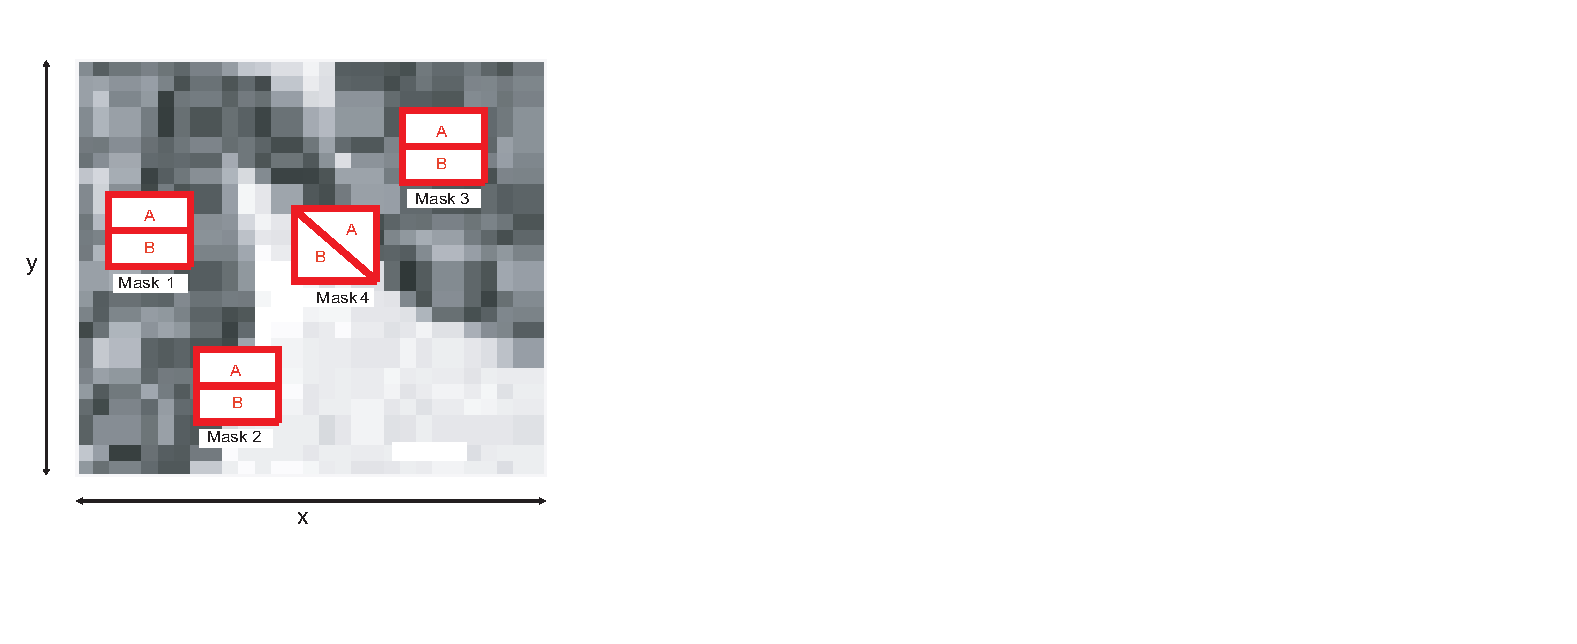
\includegraphics[scale=0.35]{2D3Dmasks1}
\caption{ Mask 1,3, not located on a boundary (low output). Mask 2 located on boundary, incorrect orientation (low output). Mask 4 located on boundary, correct orientation (high output).}
 \end{figure}
 \begin{itemize}
 \item Through a procedure of shifting the orientation of the mask, the position correlating to maximum dissimilarity then provides the output magnitude for that pixel.
 \item This process is repeated for each pixel in the image, evaluating the location, strength, and orientation of edges present in an image.
 \end{itemize}

\end{multicols}
 \end{frame}
%------------------------------------------------
\begin{frame}
\frametitle{ Problems }
The problem with Gradient and Rotational methods is that their performance on texture based interfaces is less than optimal.\\

In 2D data alone, it has been shown that 2D statistical based methods outperform traditional gradient based detection where excessive texture is evident in the image, or when the intensity profile of an edge is weaker.

		\begin{figure}
		
			\begin{tabular}{c c c}
			
					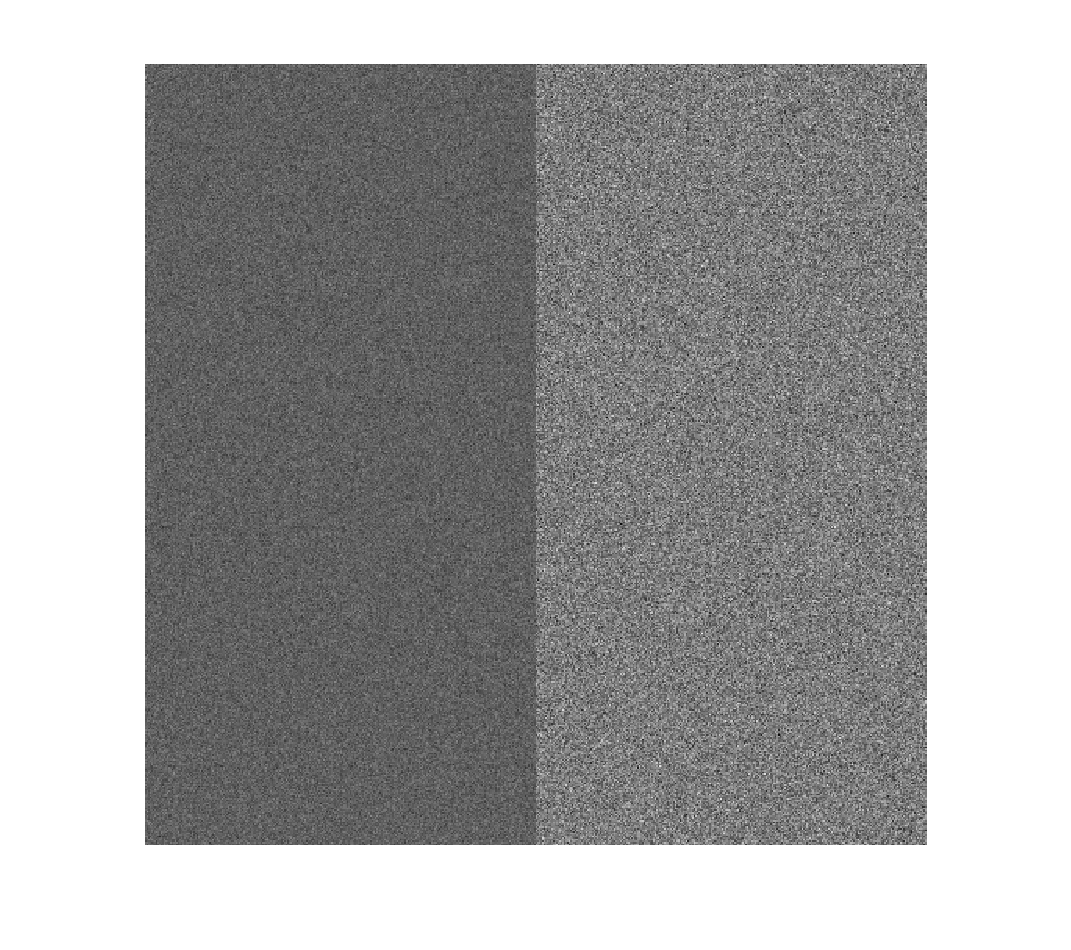
\includegraphics[scale=0.2]{newstatinterface} &

					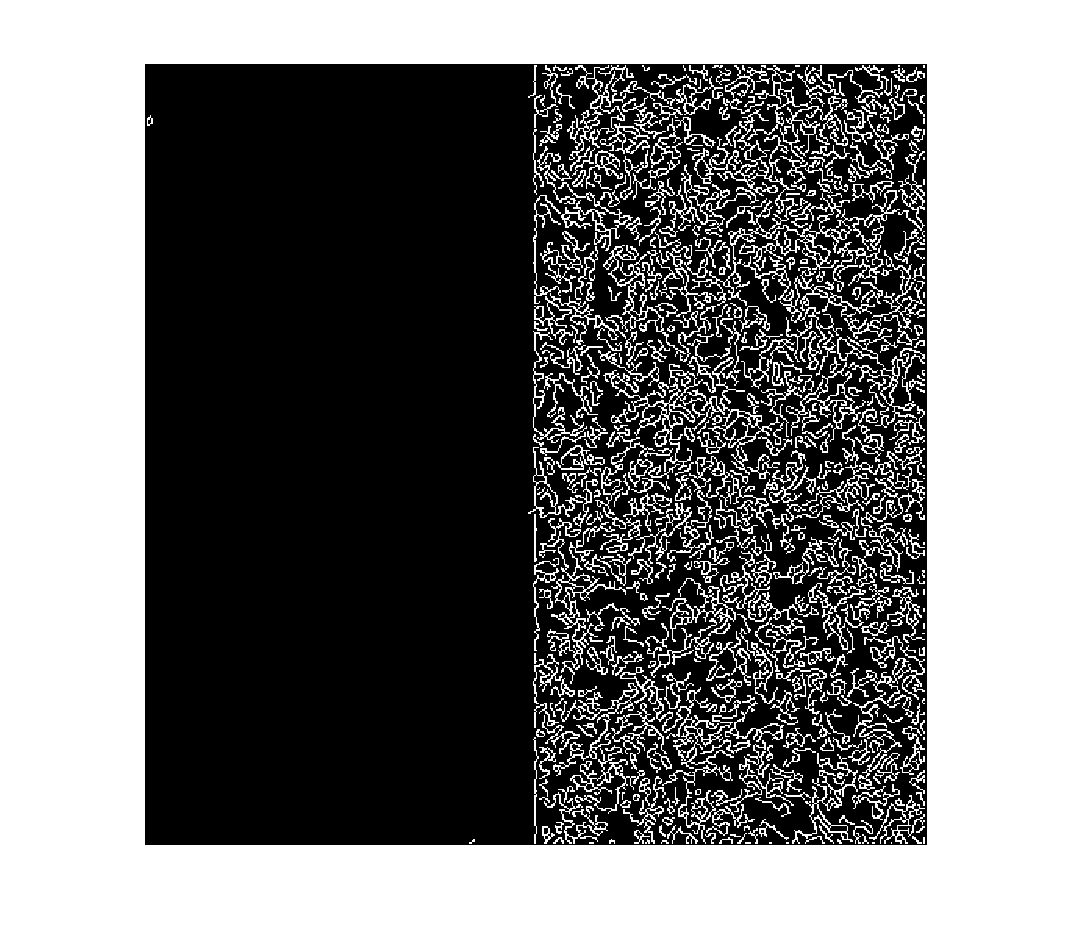
\includegraphics[scale=0.2]{cannyfail1} &
	
					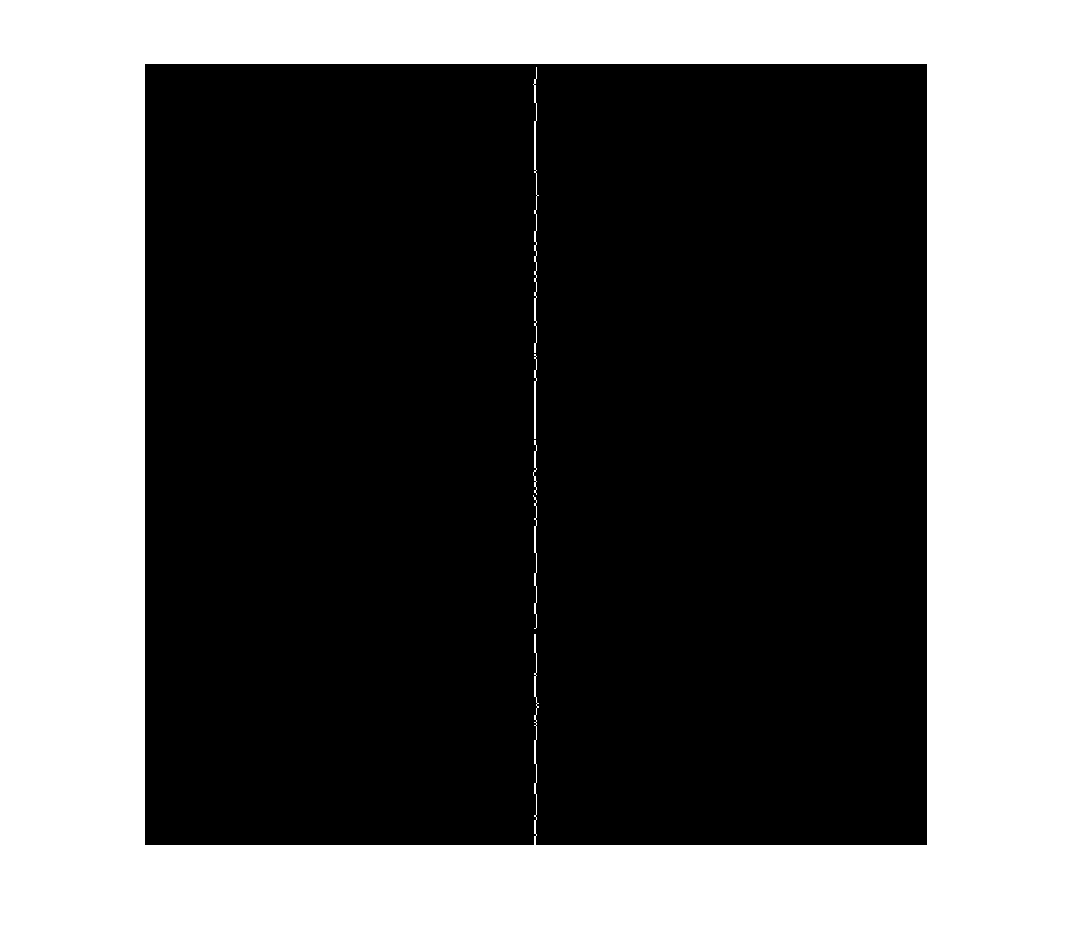
\includegraphics[scale=0.2]{ks2d}\\
	
					a & b & c
			

			\end{tabular}			
		
					\caption{a) Noisy/texture interface. b) Output from 2D Canny method. c) Output from 2D Statistical edge detection }

		\end{figure}	

\end{frame}

\section{Statistical Model}
	\begin{frame}
			\frametitle{Statistical Surface Detection Model}

Extending upon the two dimensional statistical edge detection method, a model for detecting surfaces can be produced.

The model should be able to:
				\begin{itemize}
						\item Detect surfaces in three dimensional image volumes.
						\item Locate interfaces that lie in the plane of the surface operator.
						\item Determine interfaces at multiple intensity scales.
						\item Be robust to noise and image artefacts. 
				\end{itemize} 

	\end{frame}

%------------------------------------------------
 \begin{frame}
 \frametitle{ Statistical Surface detection}
For this work, 2 methods of surface detection were developed.
 \begin{itemize}
 \item Maximum Response method.
 \item Vector Magnitude method
 \end{itemize}
 \end{frame}
 
 \subsection{Maximum Response}
 \begin{frame}
\frametitle{ Maximum Response Method}
This method is a direct extension of 2D statistical edge detection into 3D.\\
\begin{itemize}
\item Here, voxel intensity values are extracted using a simple 3D neighbourhood mask applied across several 2D image slices. 
\item The mask is divided into two sample regions, to which a statistical test is applied measuring dissimilarity.
 \end{itemize}
 \begin{figure}
 \begin{tabular}{c c}
 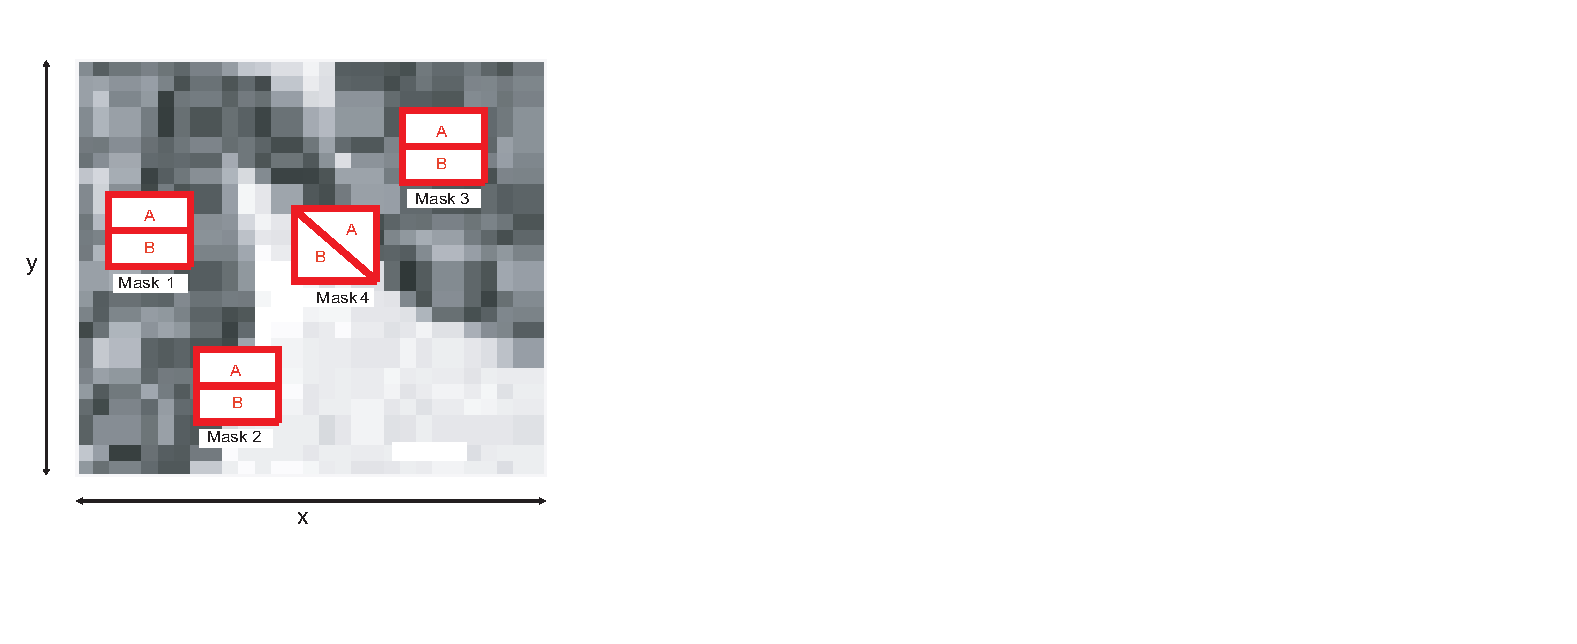
\includegraphics[scale=0.25]{2D3Dmasks1}& 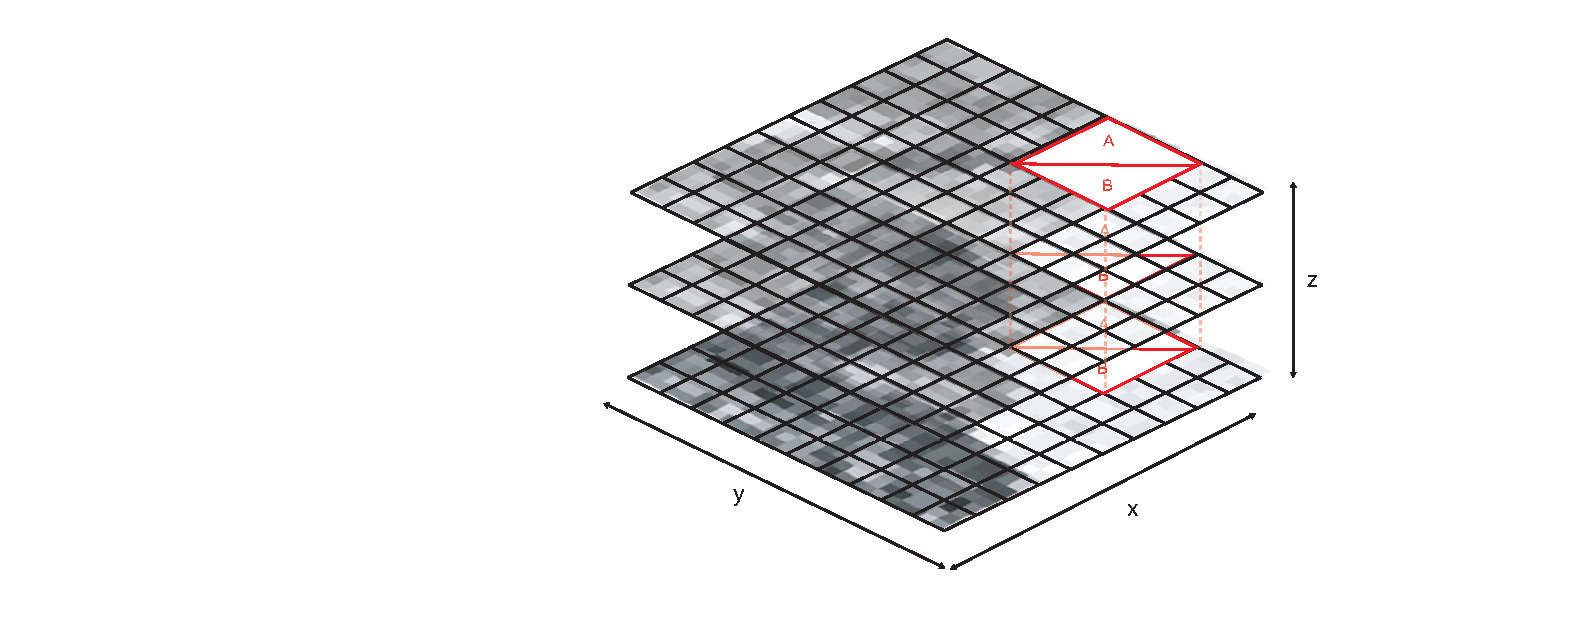
\includegraphics[scale=0.25]{2D3Dmasks2}
 \end{tabular}
 \end{figure}
 \begin{itemize}
 \item Through a procedure of shifting the orientation of the mask, the position correlating to maximum dissimilarity then provides the output magnitude for that voxel.
 \item This process is repeated for each voxel in the image, evaluating the location, strength, and orientation of surfaces present in a 3D image.
 \end{itemize}
 \end{frame}
\begin{frame}
\frametitle { Maximum Response Method }
\begin{itemize}
\item This method selects orientations based on a 26-connectivity neighbourhood.
\item If we define a single orientation as the direction from the central neighbourhood voxel to a neighbouring voxel, due to the rotational symmetry of the mask, half of the positions would be redundant as the same output would be provided.
\item Therefore this method computes 13 orientations.
\end{itemize}
\begin{figure}
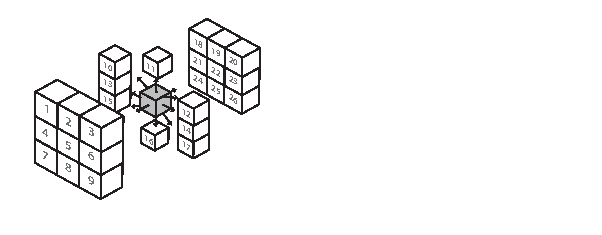
\includegraphics[scale=0.8]{cubeAngles13}
\caption{ 26 connectivity Neighbourhood mask}
\end{figure}
\end{frame}
 
%------------------------------------------------
 \subsection{Vector Magnitude}
\begin{frame}
\frametitle{Vector Magnitude}
\begin{itemize}
\item Alternatively, a statistical test can be applied in 3 orientations, across the $x$,$y$ and $z$ Cartesian planes.
\end{itemize}
\begin{figure}
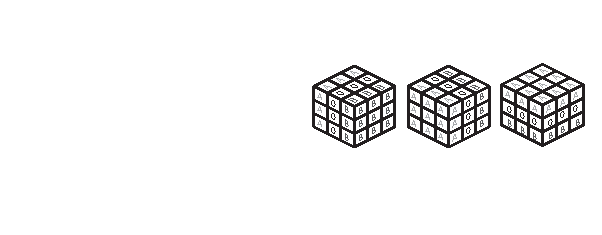
\includegraphics[scale=0.8]{cubeAngles3}
\caption{Vector Magnitude Method}
\end{figure}
\end{frame}
\begin{frame}
\frametitle{ Vector Magnitude}

The outputs of the statistical tests in each orientation provide a vector of dissimilarity.\\

		\begin{equation}
				V= T_{x}\hat{i}+T_{y}\hat{j}+T_{z}\hat{k}
		\end{equation}
		
		Where $T_{x}$,$T_{y}$,$T_{z}$ are the magnitude components of the vector V, provided by the output of a statistical test measure of dissimilarity between neighbourhood regions  The overall magnitude can then be computed by finding the Euclidean norm, defined as:\\
			\begin{equation}
				\|x\| = \sqrt{{T_{x}}^{2}+{T_{y}}^{2}+{T_{z}}^{2}}	
			\end{equation}	
	 By computing the the Ecludian norm over 3 orientations, instead of determining the maximum response of 13 orientations, it becomes significantly less computationally expensive.

\end{frame}



\subsection{Neighbourhood Masks}
	\begin{frame}
			\frametitle{Neighbourhood Mask}

				\begin{itemize}
			
					\item The mask neighbourhood is of equal scale in 3 dimensions
					\item To centralise the neighbourhood mask around a voxel, the mask length in each direction must be an odd value.
					\item When choosing a suitable size for a neighbourhood mask, there is a trade off between reliability and accuracy
				\end{itemize}	
				
	\end{frame}	
	
	\subsection{Mask Scale}
	%----------------------------
	\begin{frame}
			\frametitle{Mask Scale}		
						\begin{block}{\textbf{As mask size increases}	}
						
								\begin{itemize}
									\item Improved resolving power.
									\item Greater suppression of noise.
									\item Less susceptible to image artefacts.
									\item Image details smaller than the neighbourhood mask are not captured.
									\item More uncertainty in the location of the interface.
									\item More computationally expensive
								\end{itemize}
						\end{block}
						\textbf{Ideally we want to keep the mask as small as possible to locate finer details, while large enough to resolve texture based boundaries}				



	\end{frame}

\subsection{Statistical Comparison Tests}
\begin{frame}
\frametitle{ Statistical test }
A key aspect which determines the effective of statistical surface detection are the statistical tests which are applied. Different regions of an image contain different statistical properties such as mean, standard deviation, skewness and kurtosis, as well as feature descriptors such as those identified by Haralick. These features combine together to define the intensity and texture profile of a region.\\



\end{frame}
\begin{frame}
\frametitle{ Student's T test }
\begin{columns}
\column{.40\textwidth} 	
In probability theory, the first and second moments of a probability density function are mean and variance, therefore these two properites play a fundamental role in describing image region characteristics. The Student T test is a popular mean based statistical test which tests the hypothesis that two distributions will have a similar mean value.
\column{.40\textwidth} 	
\begin{block}{ $T$-test}
			\begin{equation}
				T = |\bar{x}_{A} - \bar{x}_{B}|\sqrt{\frac{N-1}{\sigma_{A}^{2} + \sigma_{B}^{2}}}
			\end{equation}
		Where $\bar{x}_{A}$, $\sigma_{A}^{2}$ and $\bar{x}_{B}$, $\sigma_{B}^{2}$ are respectively the mean and variance of mask regions A and B, and N is the number of pixels in each single region. 
		\end{block}
		\end{columns}
\end{frame}

\begin{frame}
\frametitle{ Difference of Boxes }
\begin{columns}
\column{.40\textwidth} 	
The Difference of Boxes test is the second mean based test used in this work. It's simply the absolute difference of the means of each region. This method provides similar outputs to gradient based methods.
\column{.40\textwidth} 	
\begin{block}{ Difference of Boxes -test}
			\begin{equation}
				D= |\bar{x}_{A} - \bar{x}_{B}|
			\end{equation}
		Where $\bar{x}_{A}$, and $\bar{x}_{B}$ are the mean  of mask regions A and B,. 
		\end{block}
		\end{columns}
\end{frame}

\begin{frame}
\begin{columns}
\column{.40\textwidth} 	
The$\chi^{2}$ test is a rank based test which checks for the independence of the two sorted datasets. It is a comparison measure that takes the relative difference in points at the same rank position for two binned data sets.
\column{.40\textwidth} 
\frametitle{$\chi^{2}$ Test}
\begin{block}{$\chi^{2}$ Test}

\begin{equation}
\chi^{2} = \sum_{i} \frac{R_{i}-S_{i}}{R_{i} + S_{i}}
\end{equation}
Here $R_{i}$ is the number of values in \textit{bin} $i$ of region $A$, and $S_{i}$ is the number of values in  \textit{bin} $i$ of region $B$.
\end{block}
\end{columns}
\end{frame}
	\begin{frame}
			\frametitle{Two sample Kolmogorov-Smirnov test}
				
				\begin{columns}
						\column{.35\textwidth} 	

					\begin{figure}
					\vspace*{-2cm}	
							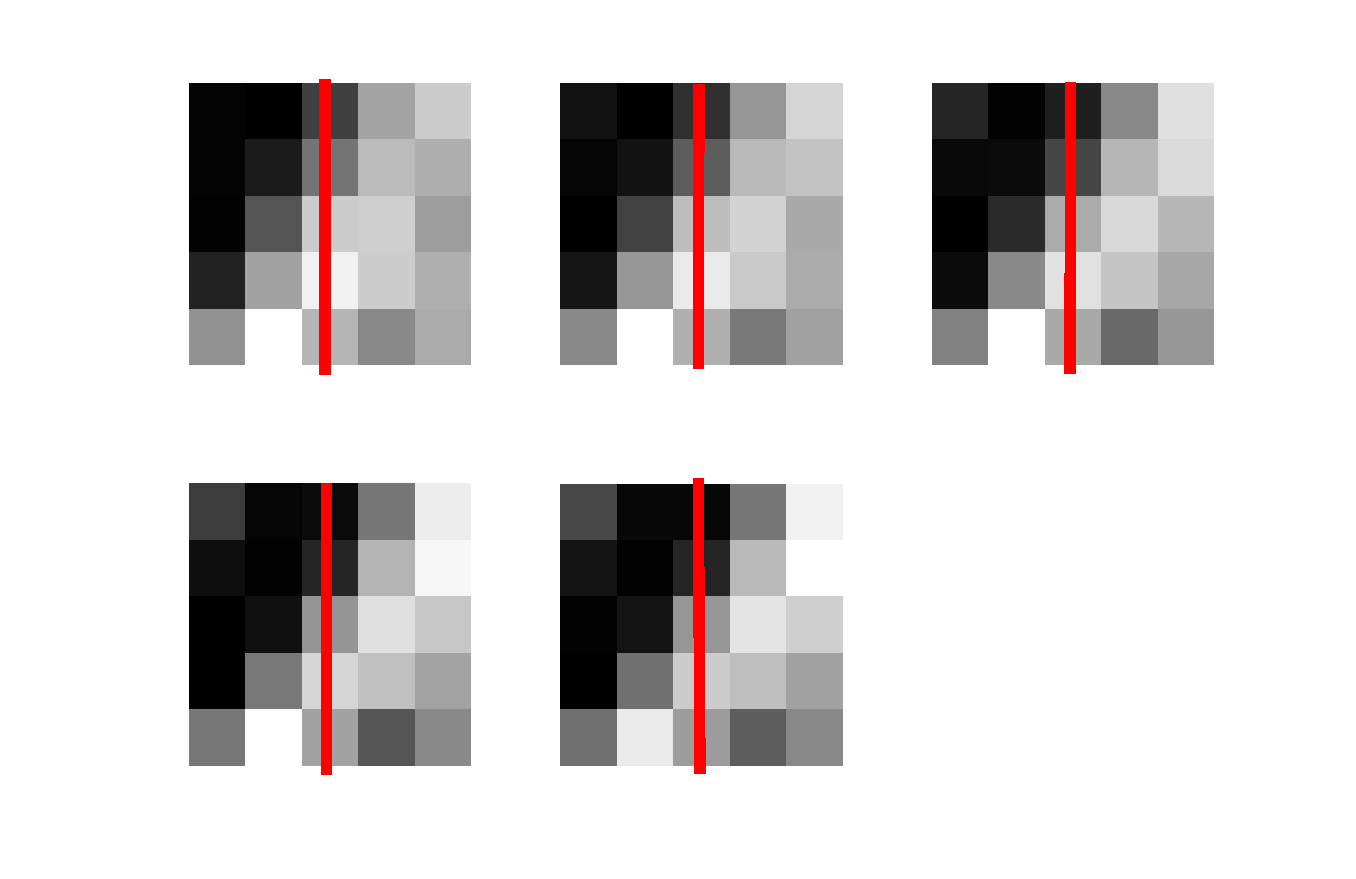
\includegraphics[scale=0.2]{kstest2sample}
					\end{figure}

Where $F_{1,n}$ and $F_{2,n}$ are the empirical distribution functions of the two samples 
						\column{.55\textwidth} 	
\begin{block}{KS-Test} 
%\vspace*{-0.5cm}	
\[  D_{n,n'} = \sup \vert F_{1,n}(x)-F_{2,n'}(y) \vert  \] 

\end{block}


					\begin{figure}
					%	\vspace*{-1cm}	
							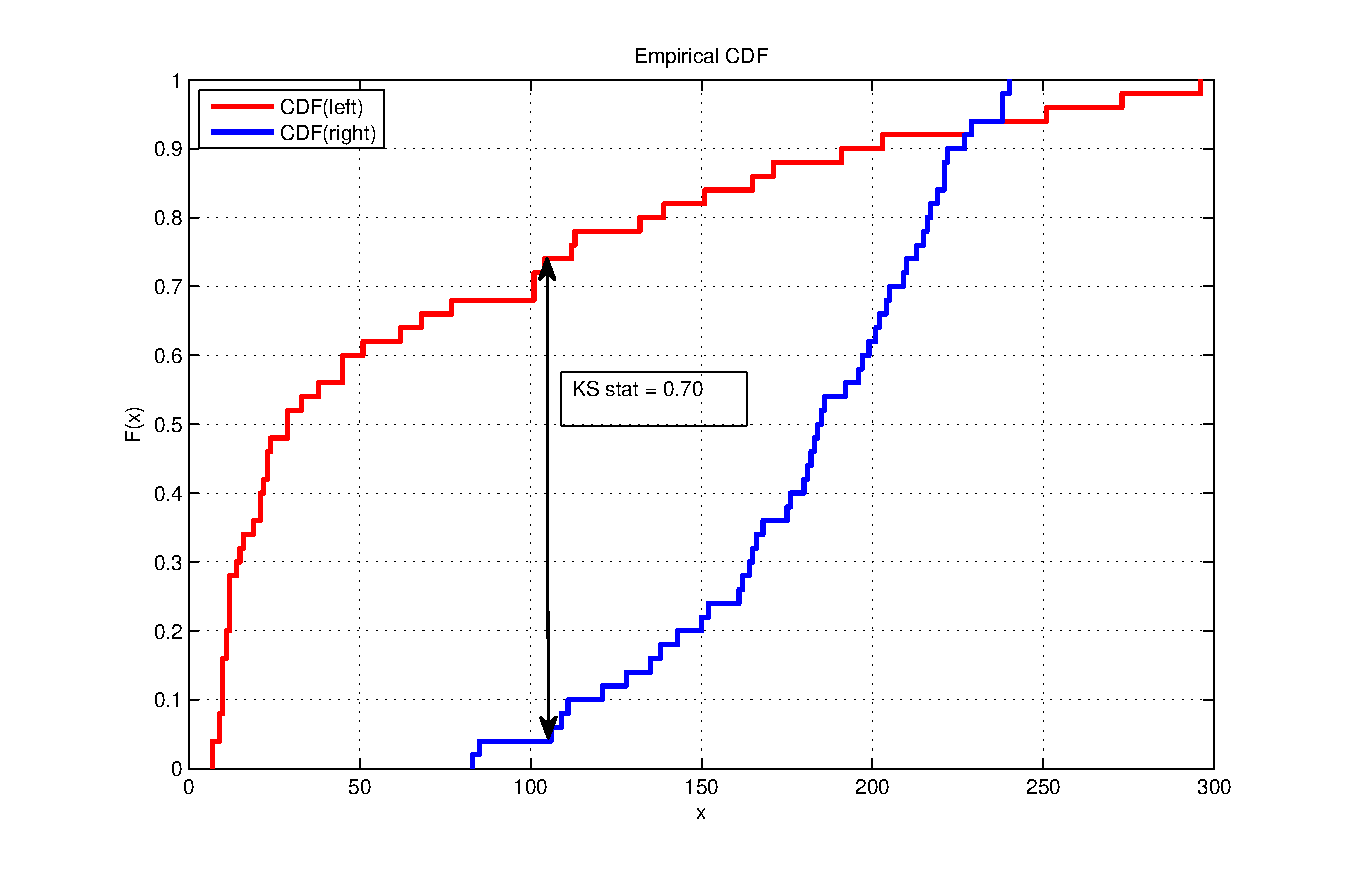
\includegraphics[scale=0.3]{cdf1}
					\end{figure}


		\end{columns}

	\end{frame}
	
	%------------------------------------------------
	
	
	\begin{frame}
			\frametitle{Two sample Kolmogorov-Smirnov test}
				
				\begin{columns}
						\column{.35\textwidth} 	

					\begin{figure}
					\vspace*{-2cm}	
							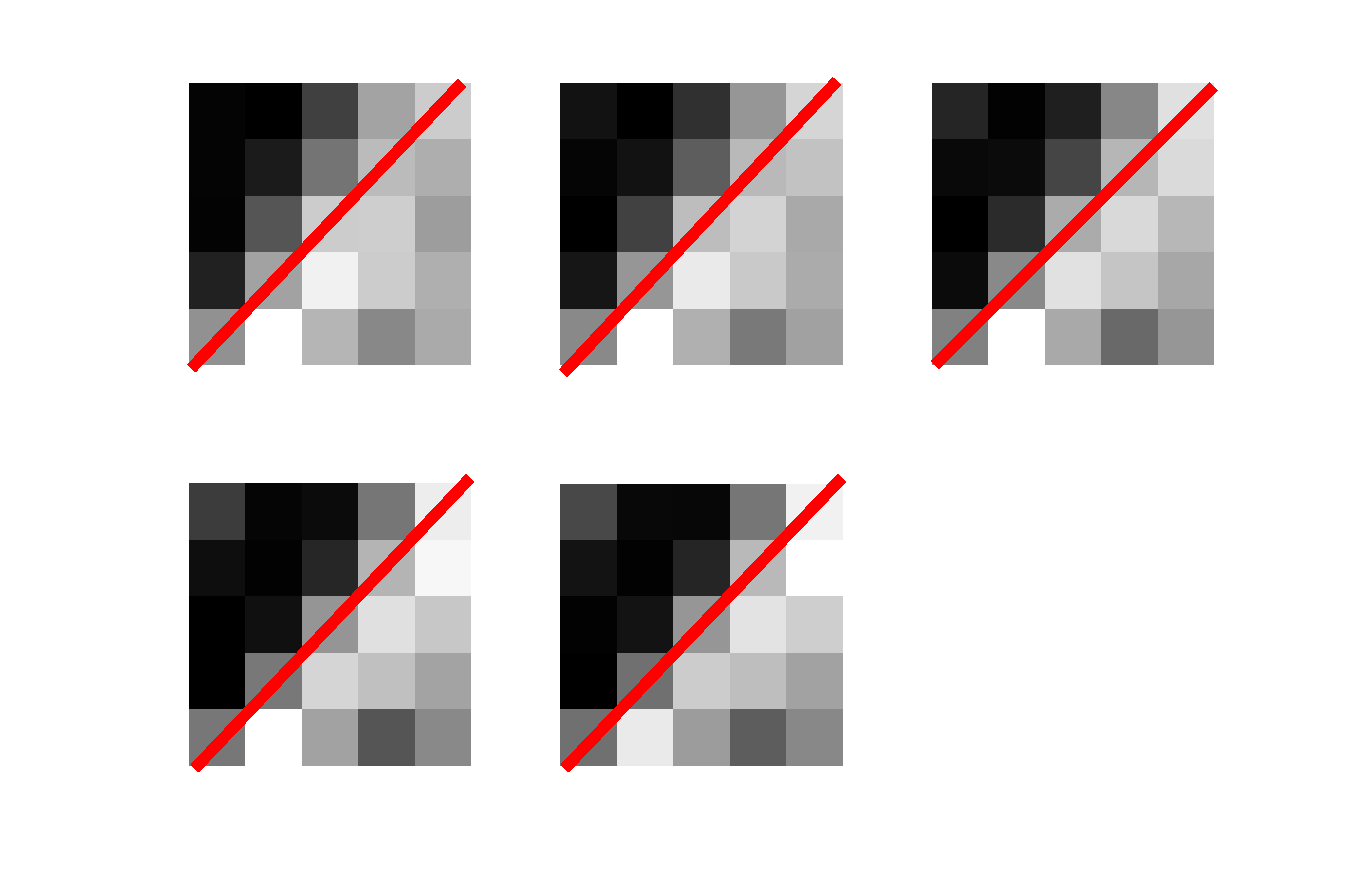
\includegraphics[scale=0.2]{kstest2sample2}
					\end{figure}

Where $F_{1,n}$ and $F_{2,n}$ are the empirical distribution functions of the two samples 
						\column{.55\textwidth} 	
\begin{block}{KS-Test} 
%\vspace*{-0.5cm}	
\[  D_{n,n'} = \sup \vert F_{1,n}(x)-F_{2,n'}(y) \vert  \] 

\end{block}


					\begin{figure}
					%	\vspace*{-1cm}	
							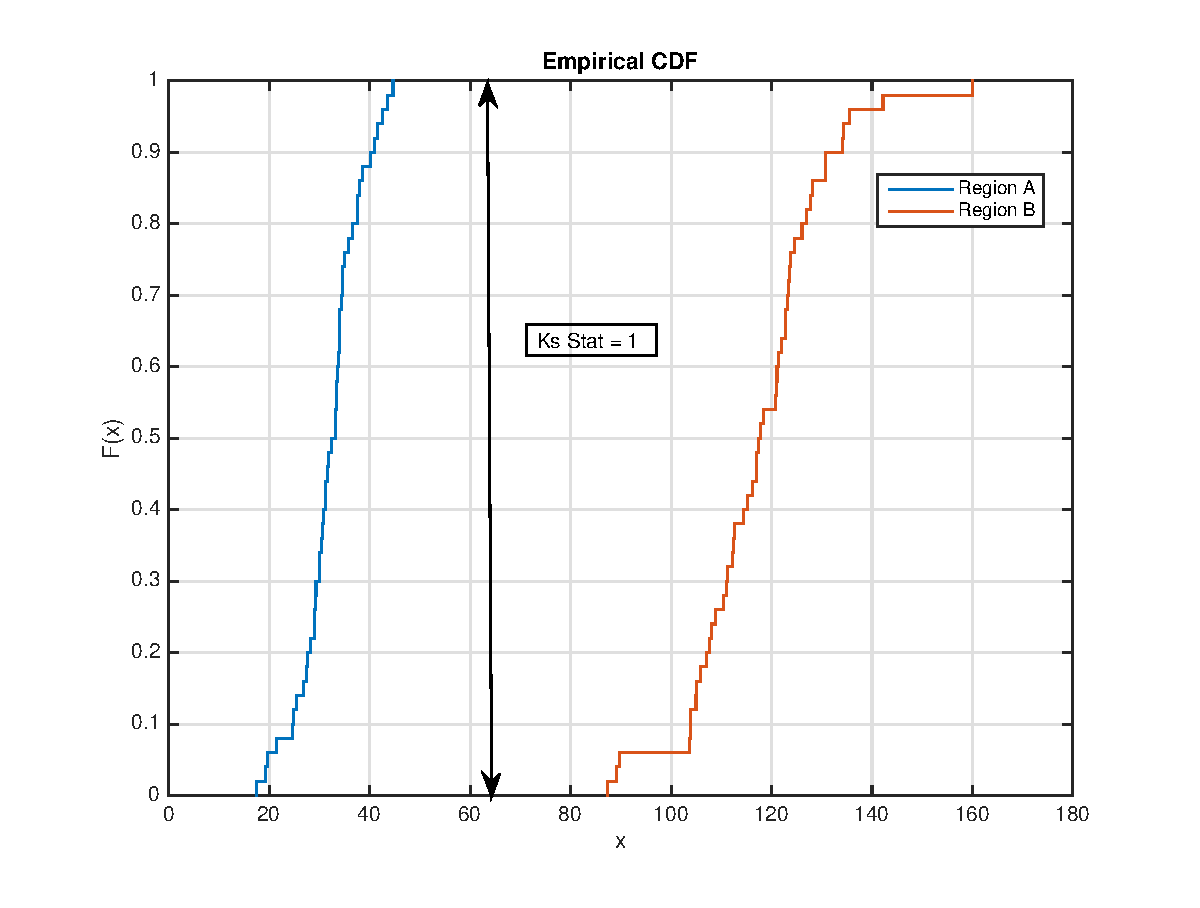
\includegraphics[scale=0.3]{cdf2}
					\end{figure}


		\end{columns}

	\end{frame}
	
	
	%------------------------------------------------


	
	\subsection{Post Processes}
%------------------------------------------------
\subsubsection{Non maximum suppression}
		\begin{frame}
			\frametitle{Non Maximum Suppression}
				
					\begin{figure}
\begin{tabular}{c c}
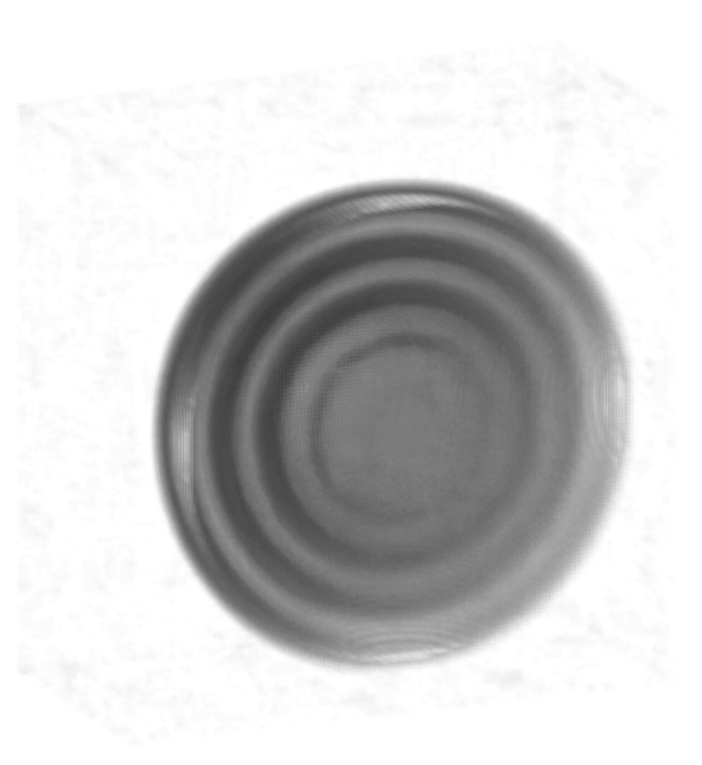
\includegraphics[scale=0.3]{outT}&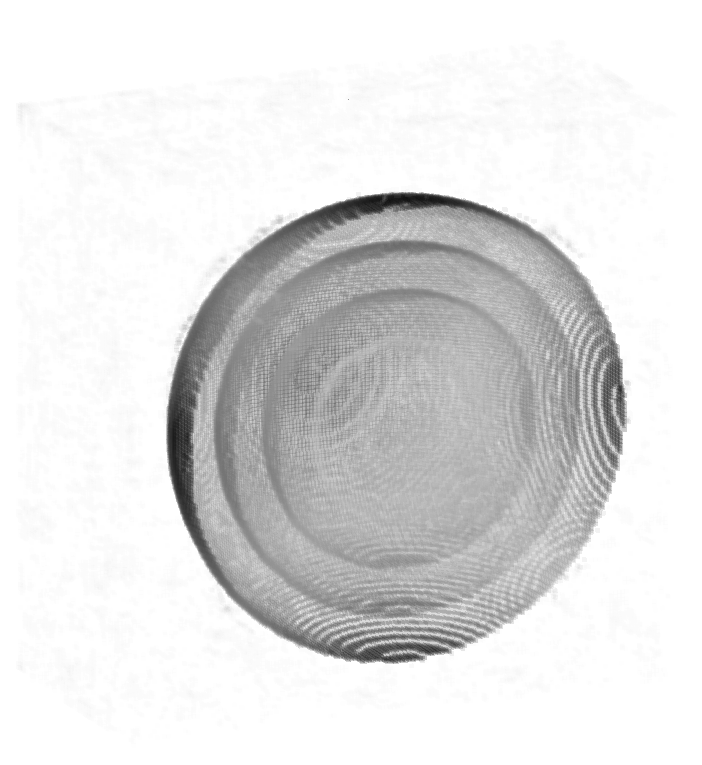
\includegraphics[scale=0.3]{outnms}\\
a & b
\end{tabular}
\caption{a) Surface map. b) Non-maximally suppressed Surface Map} 
					\end{figure}

	\end{frame}	
	\begin{frame}
			\frametitle{Non Maximum Suppression}
				
					\begin{figure}
					%	\vspace*{-1cm}	
							\includegraphics[scale=0.47]{nms}
					\end{figure}

	\end{frame}
	%------------------------------------------------

	%------------------------------------------------
	\subsubsection{Hysteresis Thresholding}
			\begin{frame}
				\frametitle{Removing Unwanted surface points}
				
					\begin{itemize}
						\item Depending on the application, not all surfaces may be required.
						\item Sometimes erroneous surfaces caused by excessive noise may be present.
						\item A simple process often used for removing these edge or surface points is Hysteresis thresholding.
						\item Hysteresis results in a logical array or binary map where edge or surface points are given the value 1, while non-edge and non-surface points are given the value 0.
					\end{itemize}		
				
			\end{frame}
%---------------------------------------------			
			
			\begin{frame}
			
			\frametitle{Hysteresis Thresholding}
			
					
						\begin{itemize}					
							\item We apply Hysteresis after non maximum suppression.
							\item It requires two threshold values. 
							\item Any surface point with an intensity greater than the upper threshold is declared an edge or surface element. 
							\item The 26 connected voxel neighbourhood surrounding a surface element is checked for intensities above the lower threshold
								\begin{itemize}
									\item Those above the lower threshold are declared  surface elements and their neighbourhoods are then checked too.
									\item Those below the lower threshold are removed
								\end{itemize}			
						\end{itemize}
				

	\end{frame}
%	%------------------------------------------------
			\begin{frame}
			\frametitle{Hysteresis Thresholding}
				
			
					\begin{figure}
						\begin{tabular}{c c c }
													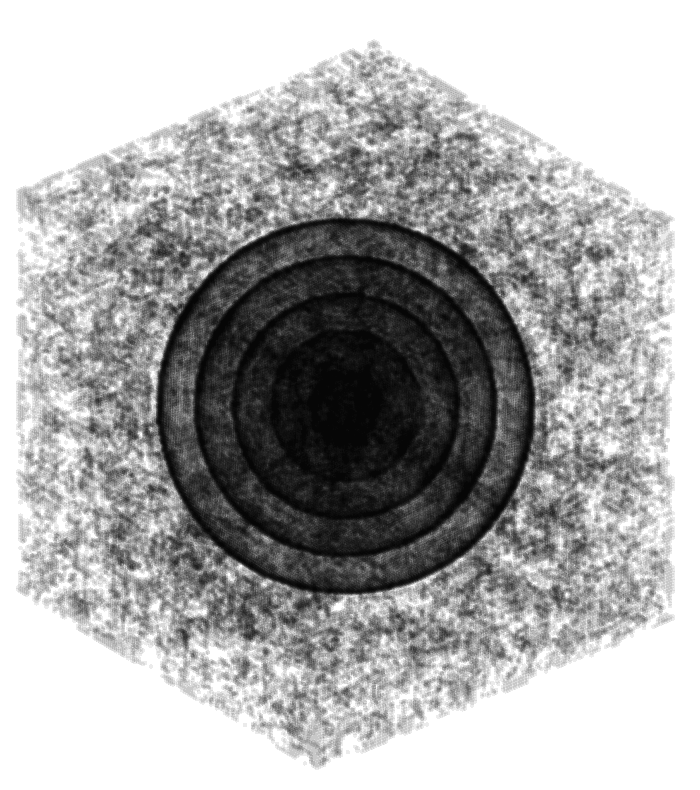
\includegraphics[scale=0.2]{Threshold50}&
													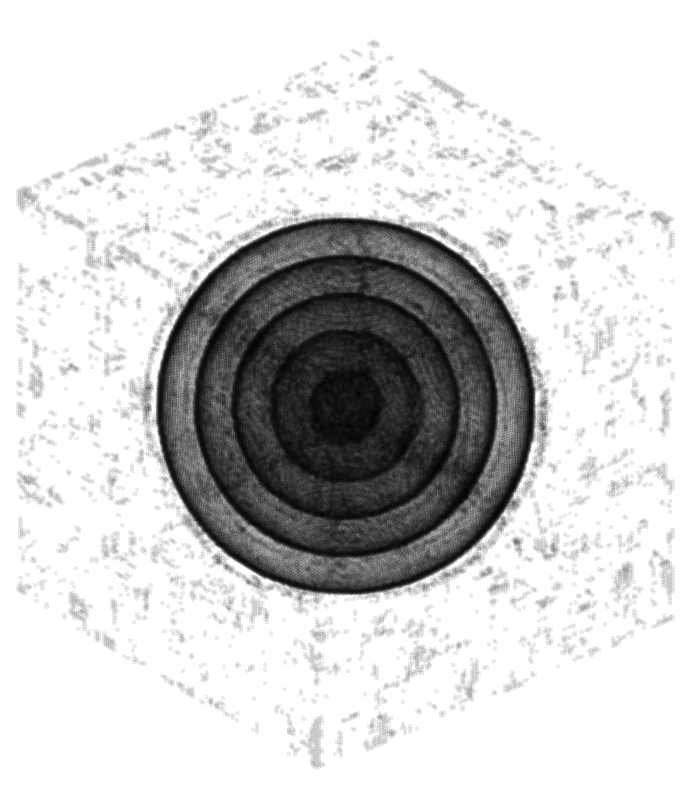
\includegraphics[scale=0.2]{Threshold75}&
													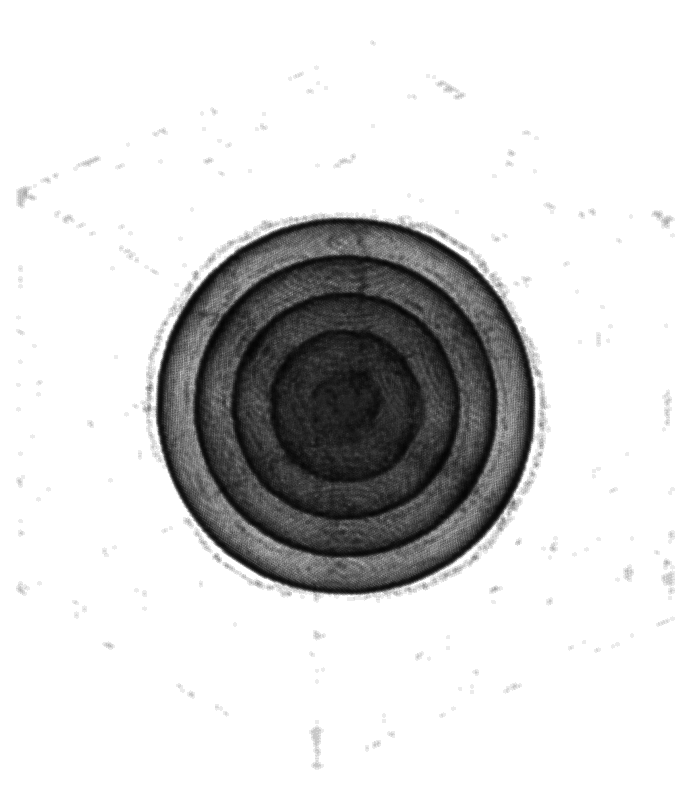
\includegraphics[scale=0.2]{Threshold100}\\
													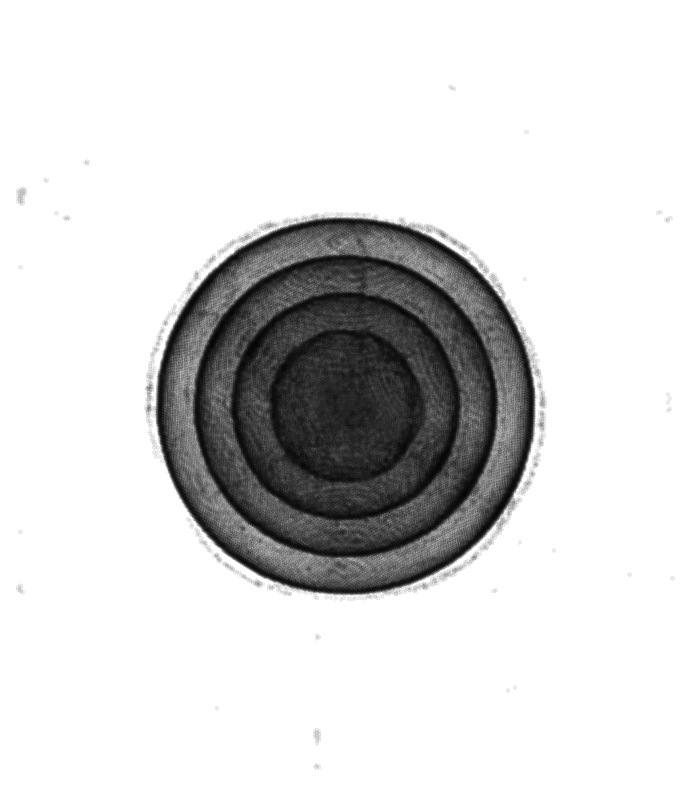
\includegraphics[scale=0.2]{Threshold125}&
													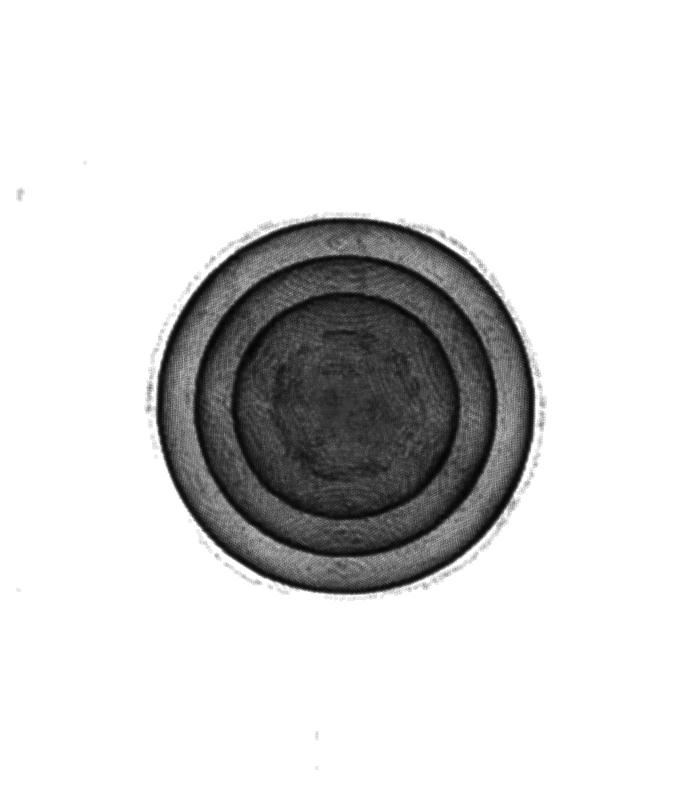
\includegraphics[scale=0.2]{Threshold150}&
													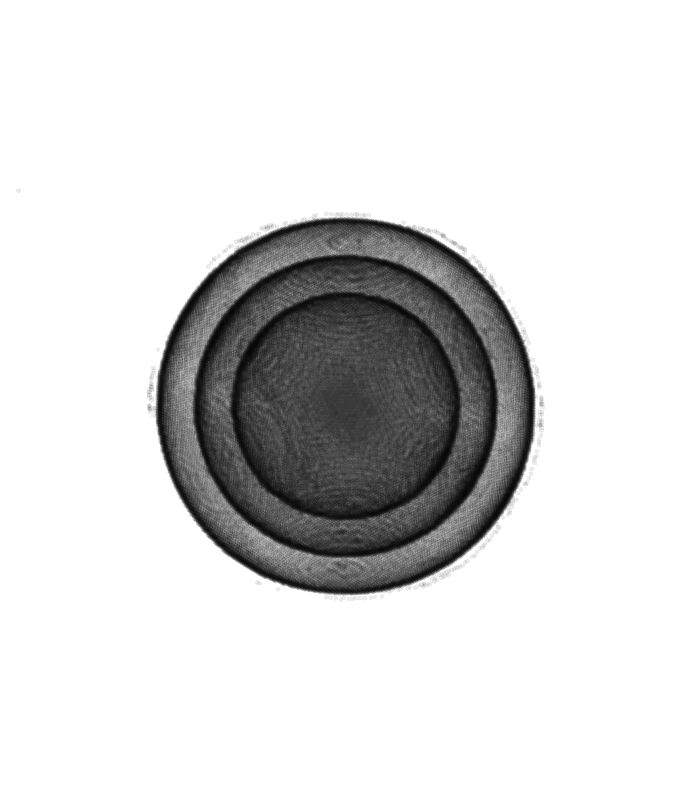
\includegraphics[scale=0.2]{Threshold200}
						\end{tabular}
\caption{Hysteresis Thresholding. Upper thresholds a) 50. b) 75. c) 100. d) 125. e) 150. f) 200. Lower threshold set to 40\% of upper}
					\end{figure}
			

	\end{frame}
	%------------------

	
\addtocontents{toc}{\newpage} % Split table in contents into second column here (requires 2 refreshes)	
\section{Methodology}

	\subsection{Types of Performance Measures}
		\begin{frame}
				\frametitle{Performance Measures}
			 			\begin{itemize}
			 			\item Qualitative 
			 			\item Quantitative
			 			\item Hybrid
			 			
			 			\end{itemize}
	\end{frame}		
		\begin{frame}
				\frametitle{Quantitative Performance Measures}
			 			\begin{itemize}
			 			\item Pratt Figure of Merit (PFOM)
			 			\item Receiver operating characteristic curves (ROC)
			 			\item Precision Recall
			 			\item Pixel Correspondence Metric (PCM)
			 			\end{itemize}
	\end{frame}
	\begin{frame}
	\frametitle{Pratt's figure of merit}
	The 3D \emph{PFOM} 
			\begin{equation}
				PFOM_{\eta} = \frac{1}{\max(N_{I}, N_{B})} \sum_{i=1}^{N_{B}}\frac{1}{1+\alpha \times d_{i}^{2}}
				\label{eq3DPFOM}
			\end{equation}
	Where $\eta$ is the maximum ideal tolerable error allowed between voxels, and was set to allow for a displacement of 1 voxel either side of the ideal. $N_{I}$ and $N_{B}$ are the surface points in the image volume and ground truth volume, respectively, $d_{i}$ is the Euclidean distance between a detected surface voxel and the nearest voxel of the ideal, and $\alpha$ is a calibration constant set at $\alpha = 1/9$, a value established by Pratt (1979)
	\end{frame}

	\subsection{Synthetic Data Creation}
	\begin{frame}
	\frametitle{Synthetic Data Creation}
	\begin{itemize}
\item Assessing the performance of surface detection methods is non-trivial if reliant on real world image data. This is due to the fact defining a ground truth data for real imagery is near impossible, and completely dependent on the scale which which one defines the existence of a boundary.

\item By creating synthetic images, we can accurately determine the ground truth solutions.
	
	\item There are numerous considerations to be made when creating synthetic image volumes
	\begin{itemize}
	\item Topology of interface 
	\item Type of interface
	\item Number of interfaces
	\item Bias of interfaces (major / minor lines)
	\item Scale
	\item Corners
	\item Data acquisition
	\end{itemize}
	\end{itemize}
	\end{frame}
	
\begin{frame}
\frametitle{Synthetically created data - Multiple scale}
\begin{figure}
\begin{tabular}{cc}

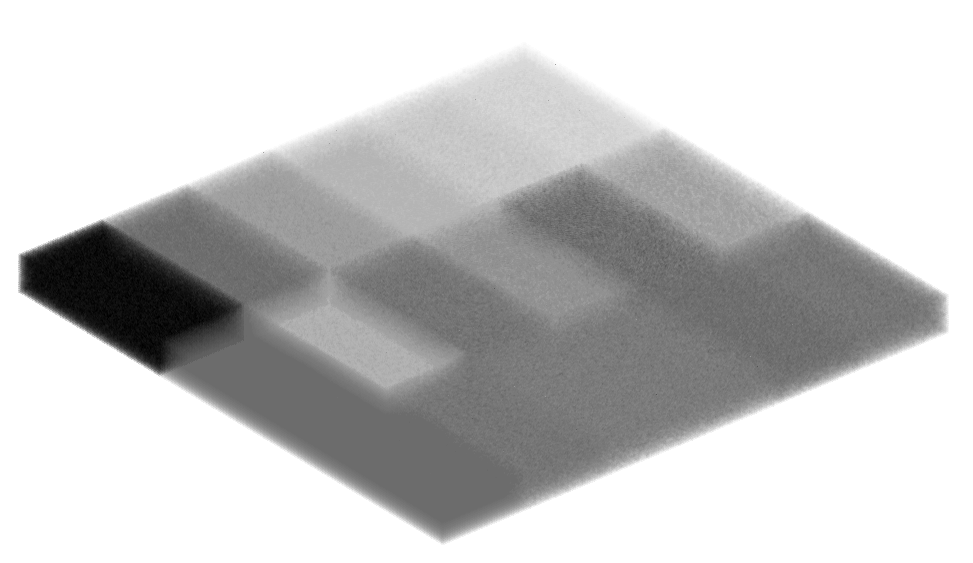
\includegraphics[scale=0.3]{multi.eps} & 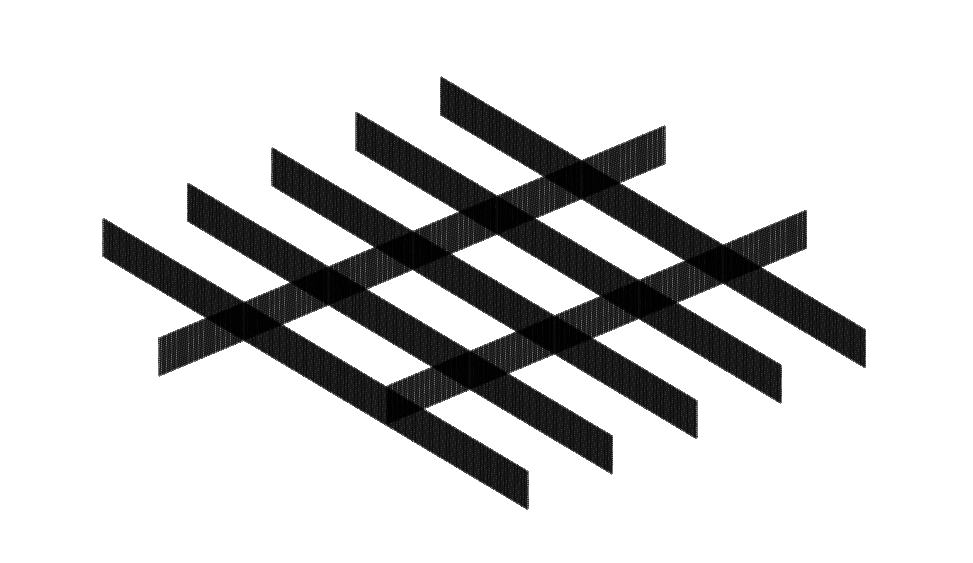
\includegraphics[scale=0.3]{multiideal.eps}

\end{tabular}
\end{figure}
\end{frame}	
	
	\begin{frame}
\frametitle{Synthetically Created Data - Multiple scale rotated}
\begin{figure}

\begin{tabular}{c c c}

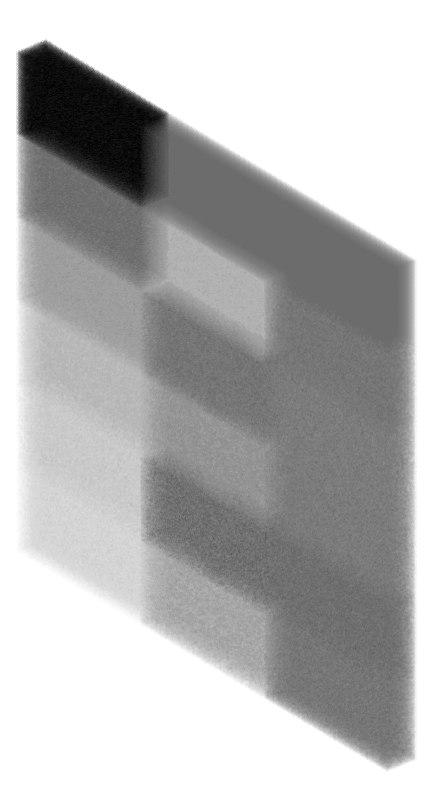
\includegraphics[scale=0.3]{multirot.eps} & &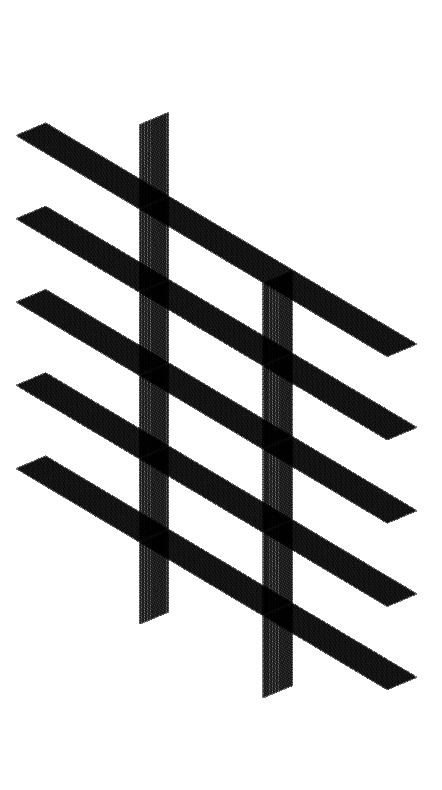
\includegraphics[scale=0.3]{multiidealrot.eps}

\end{tabular}
\end{figure}
\end{frame}	

	\begin{frame}
\frametitle{Synthetically Created Data - Multiple sphere}

\begin{figure}
\begin{tabular}{cc}

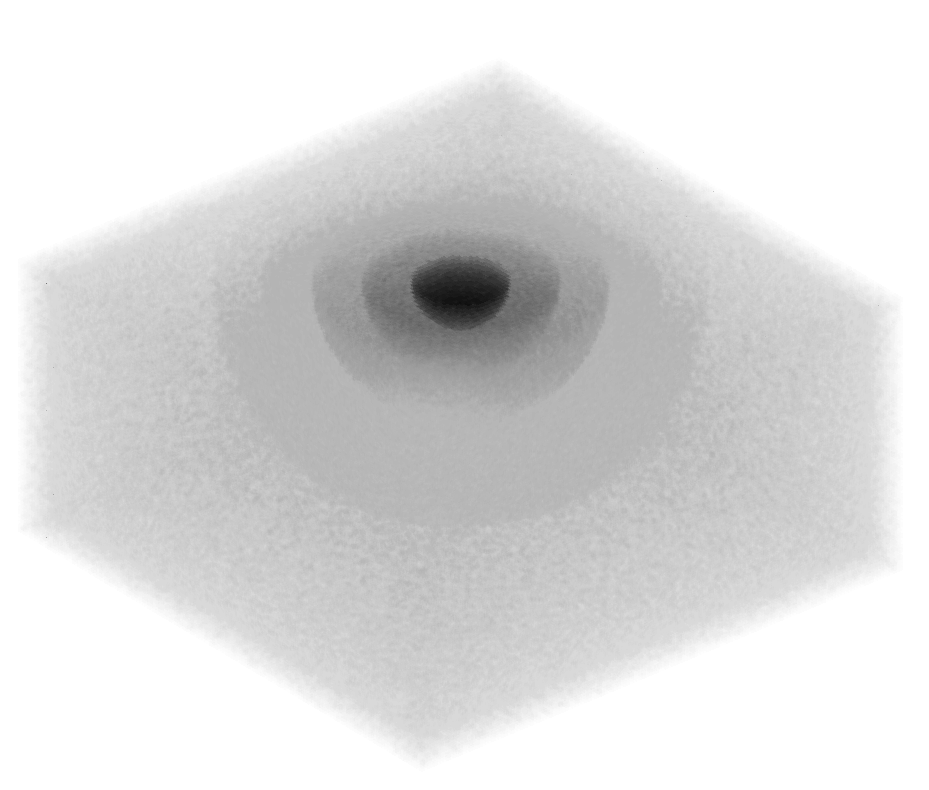
\includegraphics[scale=0.3]{sphere1.eps} & 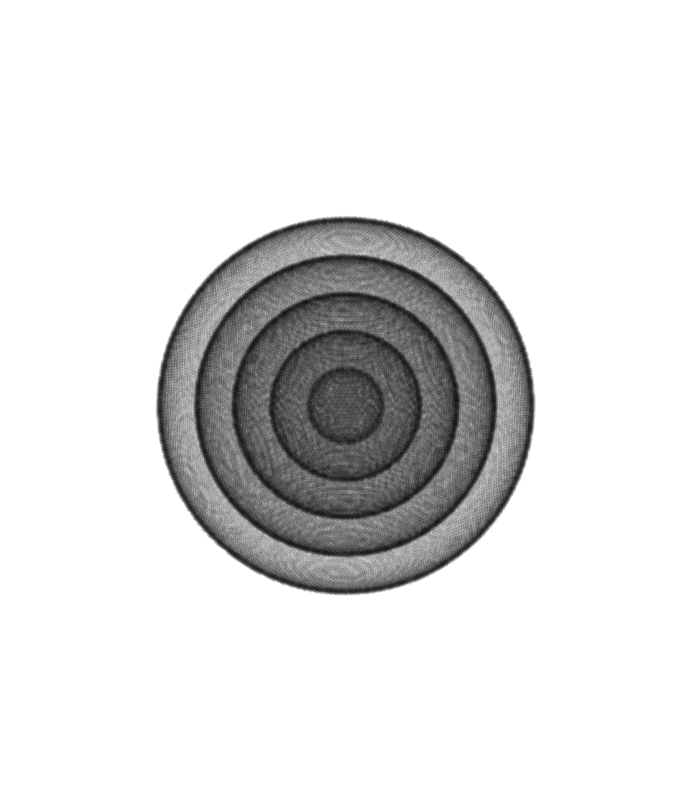
\includegraphics[scale=0.3]{sphereideal.eps}

\end{tabular}
\end{figure}
\end{frame}	

	\begin{frame}
\frametitle{Synthetically Created Data - Reverse Multiple sphere}
\begin{figure}
\begin{tabular}{cc}

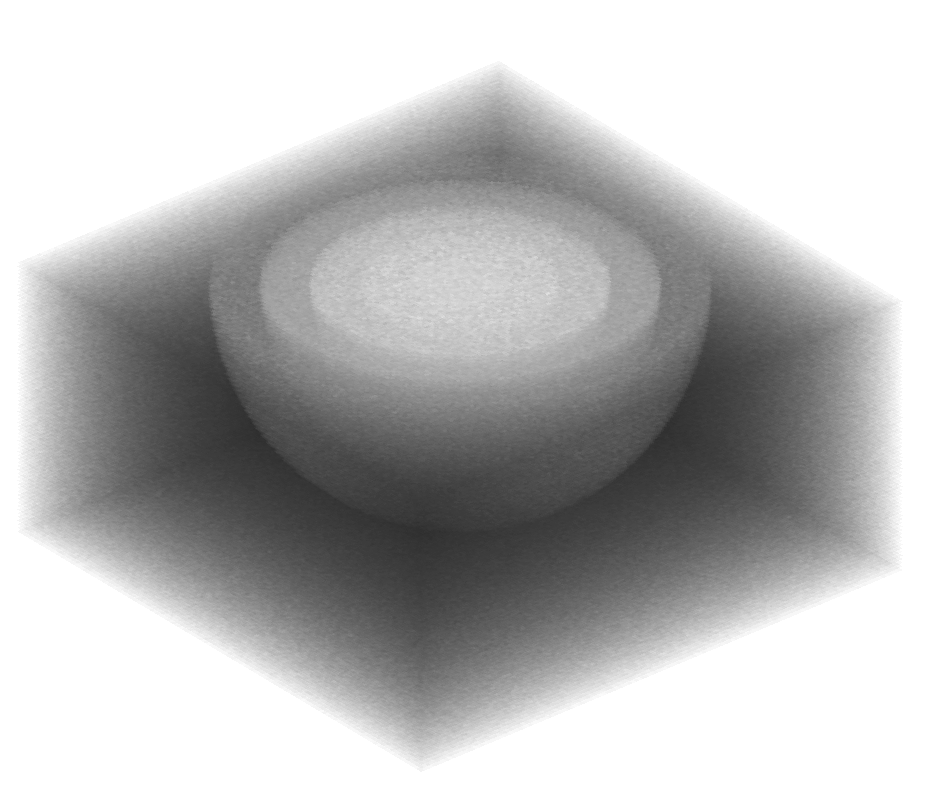
\includegraphics[scale=0.3]{sphere_reversed.eps} & 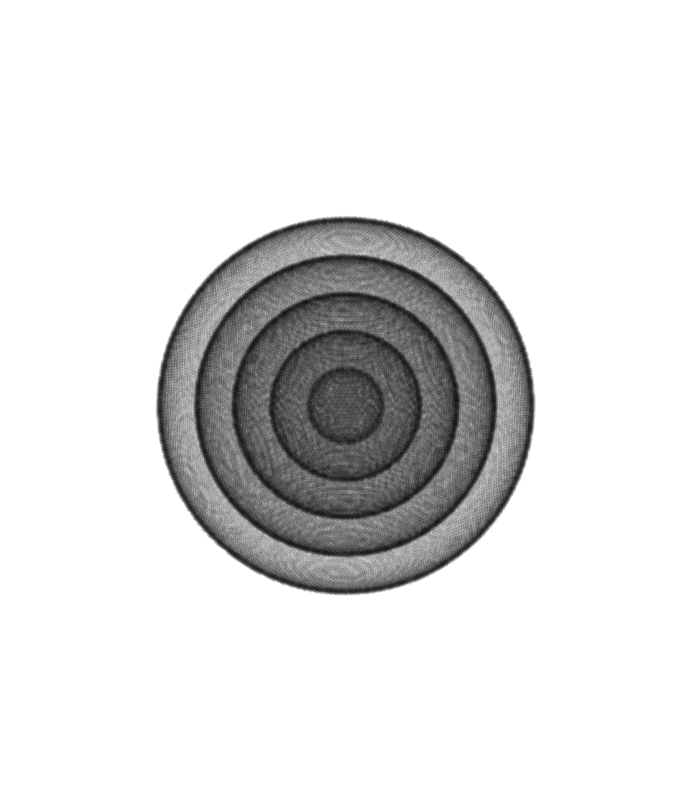
\includegraphics[scale=0.3]{sphereideal.eps}

\end{tabular}
\end{figure}
\end{frame}	

\begin{frame}
\frametitle{Synthetically Created Data - Staircase}

\begin{figure}
\begin{tabular}{c c}
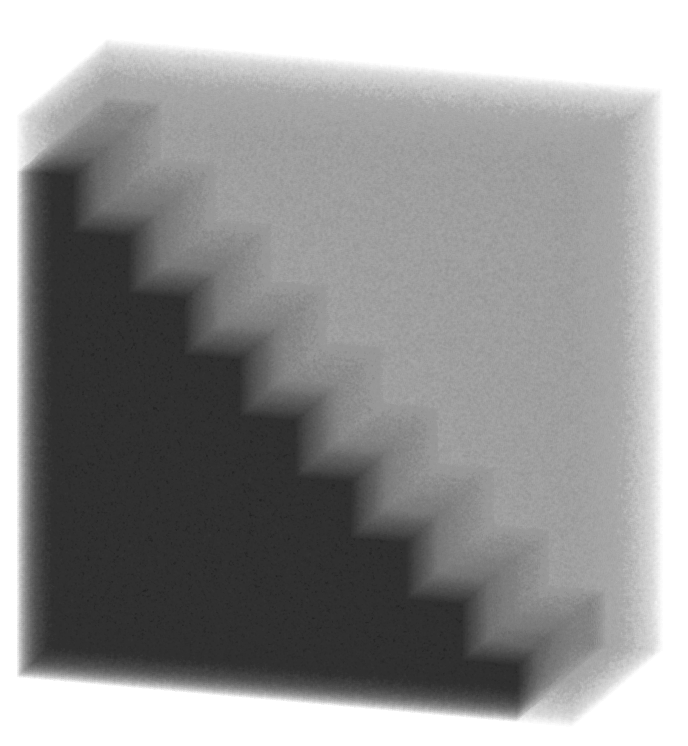
\includegraphics[scale=0.3]{staircase10.eps} & 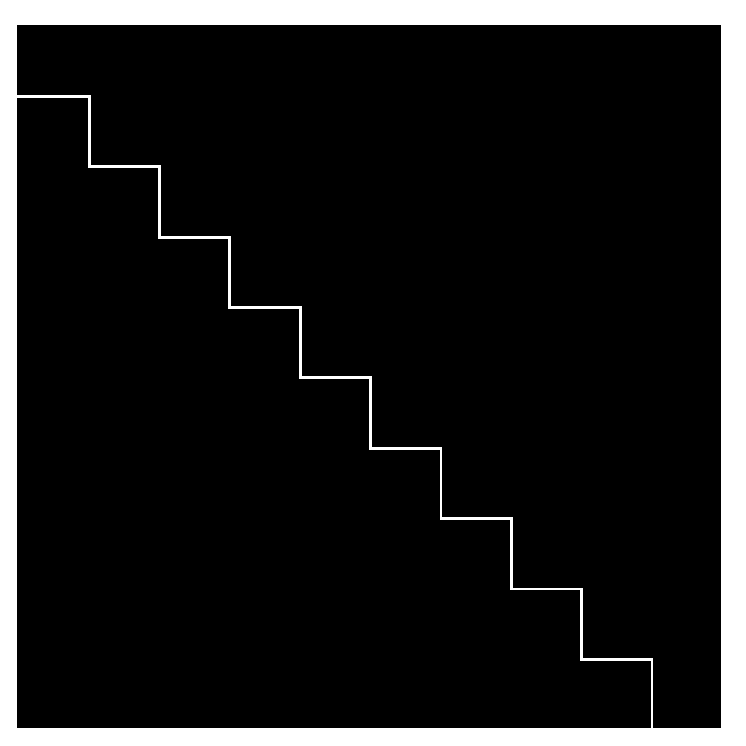
\includegraphics[scale=0.27]{staircase10ideal.eps}

\end{tabular}
\end{figure}
\end{frame}	
\begin{frame}
\frametitle{Synthetically Created Data - Staircase}

\begin{figure}
\begin{tabular}{c c}
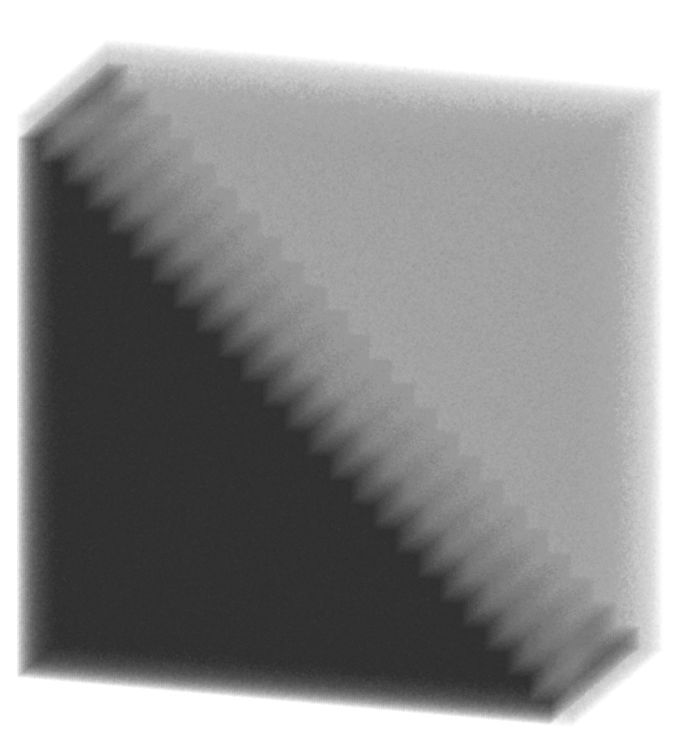
\includegraphics[scale=0.3]{staircase25.eps} & 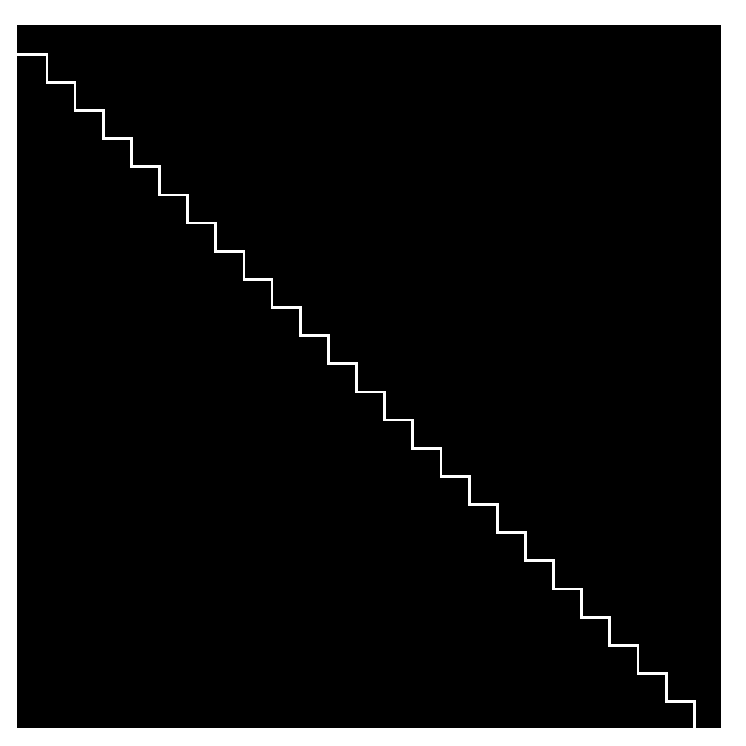
\includegraphics[scale=0.27]{staircase25ideal.eps}

\end{tabular}
\end{figure}
\end{frame}	

\begin{frame}
\frametitle{Synthetically Created Data - Cube}

\begin{figure}
\begin{tabular}{c c}
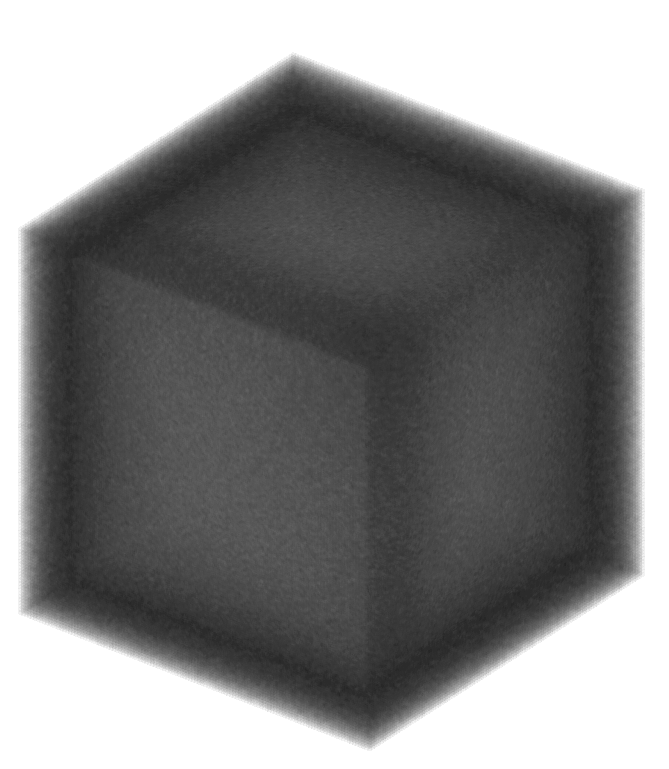
\includegraphics[scale=0.27]{cubevolume.eps}&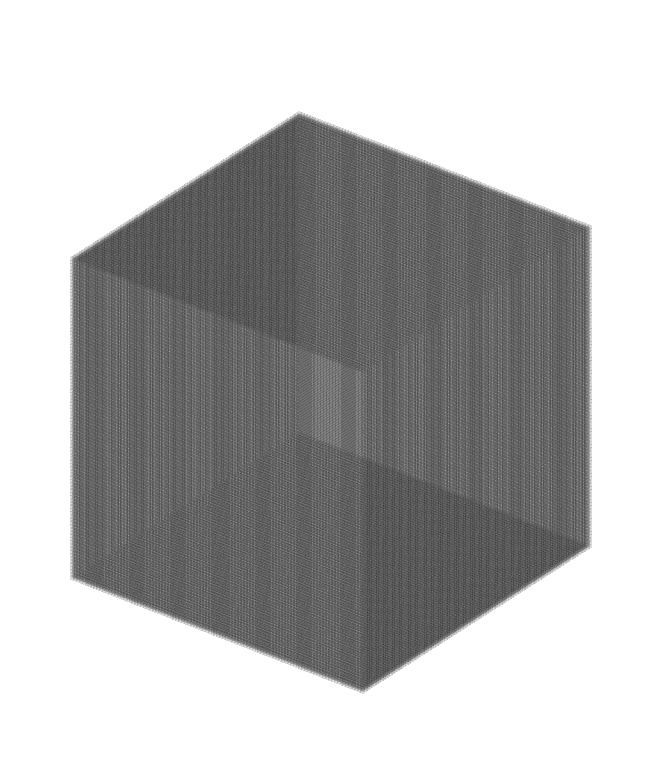
\includegraphics[scale=0.27]{cubevolumeideal.eps}

\end{tabular}
\end{figure}
\end{frame}	

\begin{frame}
\frametitle{Synthetically Created Data - Star}
\begin{figure}
\begin{tabular}{c c}
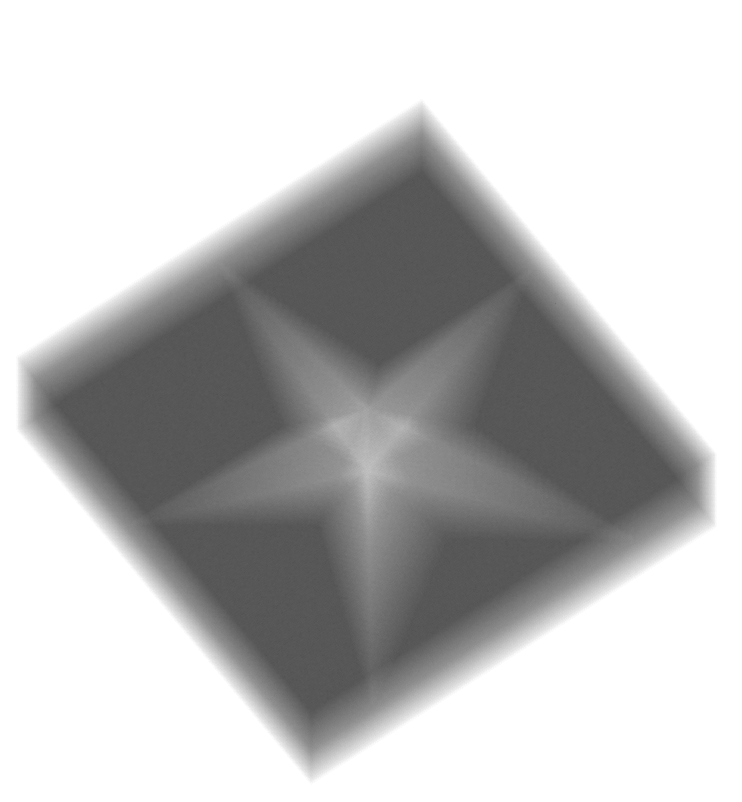
\includegraphics[scale=0.27]{star.eps}&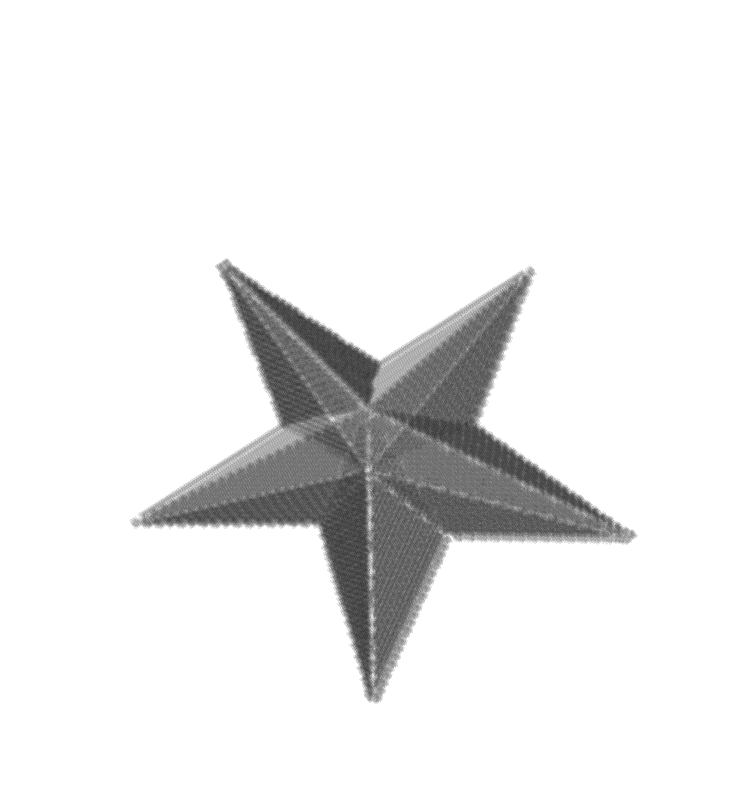
\includegraphics[scale=0.27]{starideal.eps}

\end{tabular}
\end{figure}
\end{frame}	

\subsection{Monte Carlo Analysis}

		\begin{frame}
				\frametitle{Monte Carlo Analysis}
			 			In this study we used a Monte Carlo Methodology of testing.
			 			\begin{itemize}
			 			\item Three examples of each image
			 			\item Pseudo-random values containing the same statistical properties for each image 
			 			\item Mean and standard deviation of results of each image type determines the score.
			 			\end{itemize}
	\end{frame}

\section{Results}
\subsection{PFOM scores}
	%-----------------------------
		\begin{frame}
			\frametitle{PFOM Results}
\begin{table}
    \begin{center}
        \scalebox{0.70}{
              \begin{tabular}{l l  l l| l l l l}
                        \hline
    \multicolumn{4}{l|}{Sphere $\bar{x}$ Scores   }&&&  \\
    $\sigma$ & 		2D Canny & 3D Canny& 3D Steerable & Mask Size &2D stat & 3D stat $\|x\|$ & 3D stat (max)  \\\hline
              1     &	86.28	&	92.28	&	89.60	& 5	&	78.46	&	89.88	&	91.24 \\
              2     &	87.21 	&	91.93	&	\cellcolor{green}96.92	& 7	&	84.83	&	96.90	&	97.73 \\
              3     &	 87.37	&	\cellcolor{green} 92.31	&	91.20	& 9	&	89.12	&	\cellcolor{green}98.79	&	\cellcolor{green}99.22 \\
              4     &	\cellcolor{yellow} 87.44	&	92.43	&  81.34 	& 11	&	\cellcolor{green} 92.26	&	98.46	&	99.18 \\\hline 
    \multicolumn{4}{l|}{Multiple interface }&&&  \\          
     $\sigma$ & 		2D Canny & 3D Canny& 3D Steerable & Mask Size &2D stat & 3D stat $\|x\|$ & 3D stat (max)  \\\hline
              1     & 64.86	&	70.13	&	65.07	& 5	&	72.01	&	80.64	&	80.89 \\
              2     &\cellcolor{red} 67.62 	&72.55		&	\cellcolor{yellow} 82.98	& 7	& 	84.16	&	90.23&		92.33 \\
              3     &  67.46 	&	\cellcolor{yellow}72.60	&	81.71	& 9	& 93.87	&	95.99	&	\cellcolor{green}96.17 \\
              4     &   67.35	&	72.60	&  n/a       & 11& 	\cellcolor{green} 94.16	&	\cellcolor{green}96.76	&	95.59 \\\hline
    \multicolumn{4}{l|}{Multiple interface rotated } &&& \\             
     $\sigma$ & 		2D Canny & 3D Canny& 3D Steerable & Mask Size &2D stat & 3D stat $\|x\|$ & 3D stat (max)  \\\hline
              1     &	42.72	 &	70.48	&	65.22	& 5	&	42.05	&	80.82	&	 82.57\\
              2     &	43.68	 &73.36	&	\cellcolor{yellow} 83.71	& 7	&	44.68	& 92.47	&	 92.50\\
              3     &	\cellcolor{red}43.81	 &	\cellcolor{yellow}73.43	&	82.92	& 9	& 50.02		& 	\cellcolor{green}97.02	&  \cellcolor{green}96.46\\
              4     &	43.82	 &	73.39	&     n/a		& 11	&  \cellcolor{red}52.16 	& 	96.10	&   95.90\\\hline
              \end{tabular}}\\  
    \end{center}
    \caption{\emph{PFOM} results on each test image compared to the ideal. Highlights: Poor(Red), Adequate(Yellow), Good(Green). }
   
  \end{table}   
		
			


	\end{frame}
\subsection{Visual Results}
\subsubsection{Sphere}
\begin{frame}

\frametitle{Visual Results - Sphere}

\begin{figure}
\begin{tabular}{c c c }
%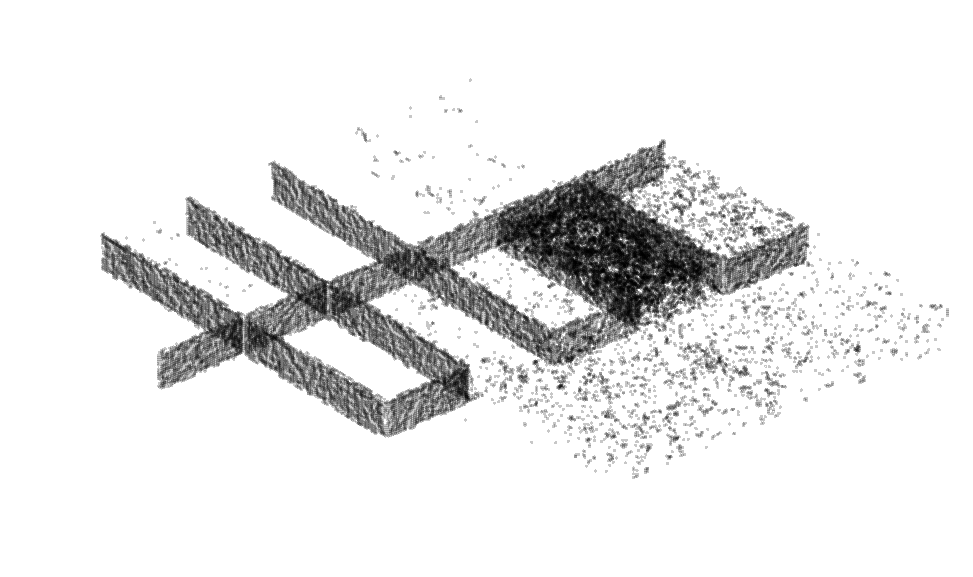
\includegraphics[scale=0.2]{Cannysigma3}&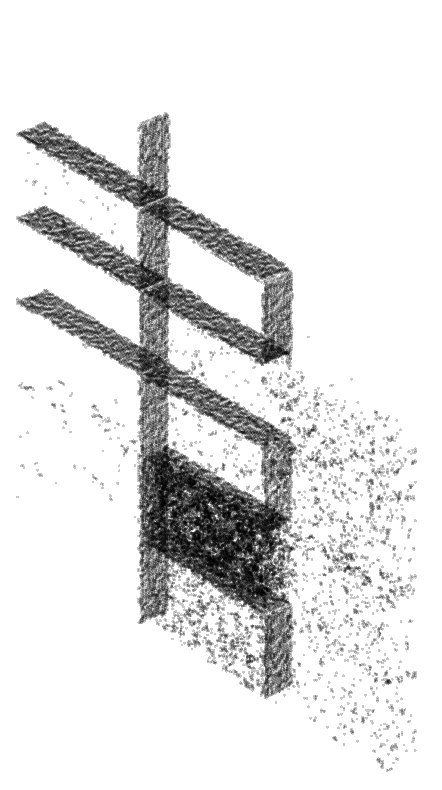
\includegraphics[scale=0.2]{Cannysigma3rot}&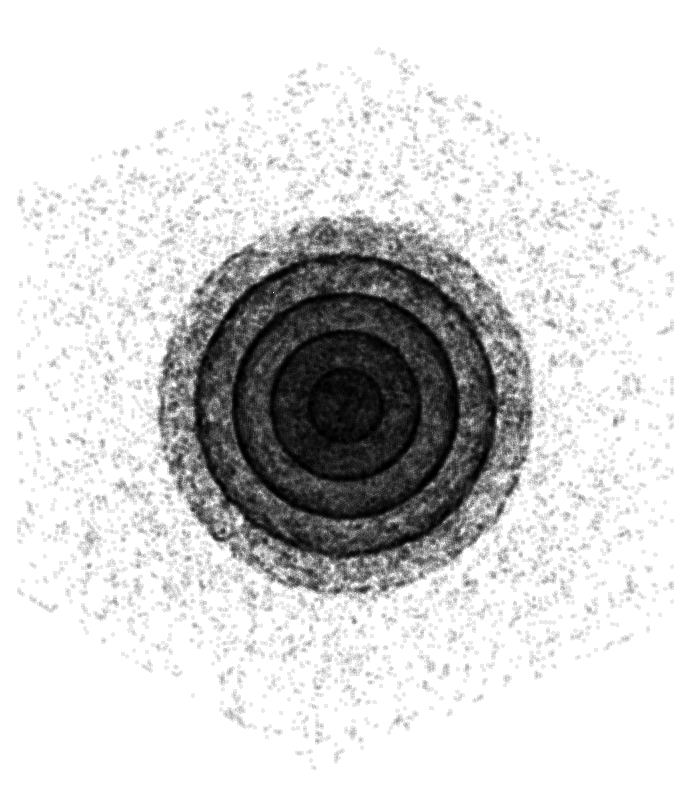
\includegraphics[scale=0.2]{Cannysigma3sphere}&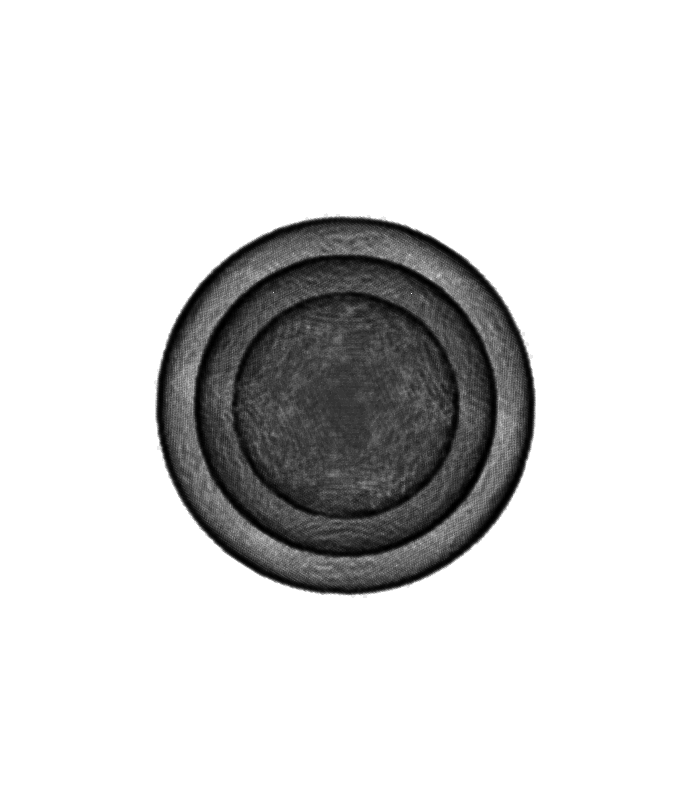
\includegraphics[scale=0.2]{Cannysigma3sphereR}\\
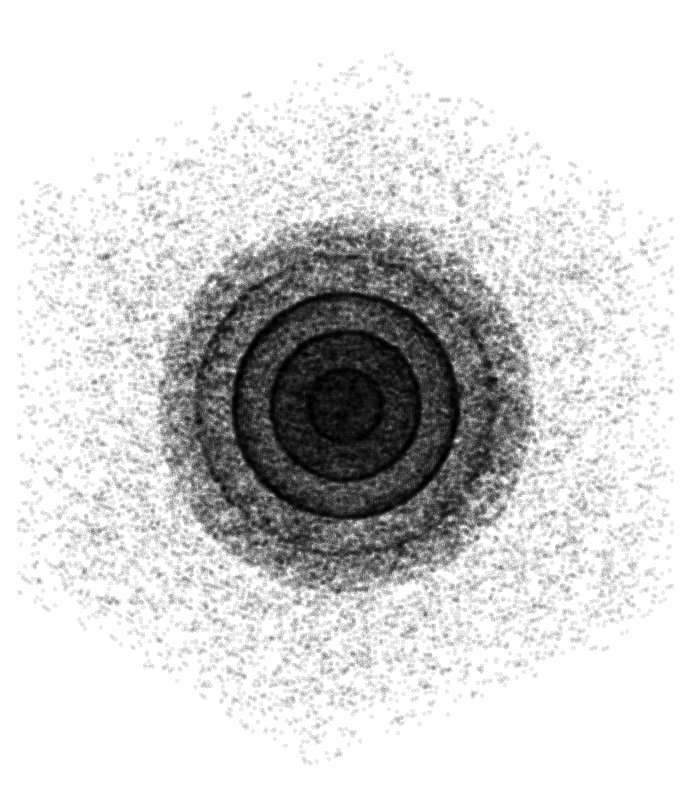
\includegraphics[scale=0.18]{canny2dsphere.eps}&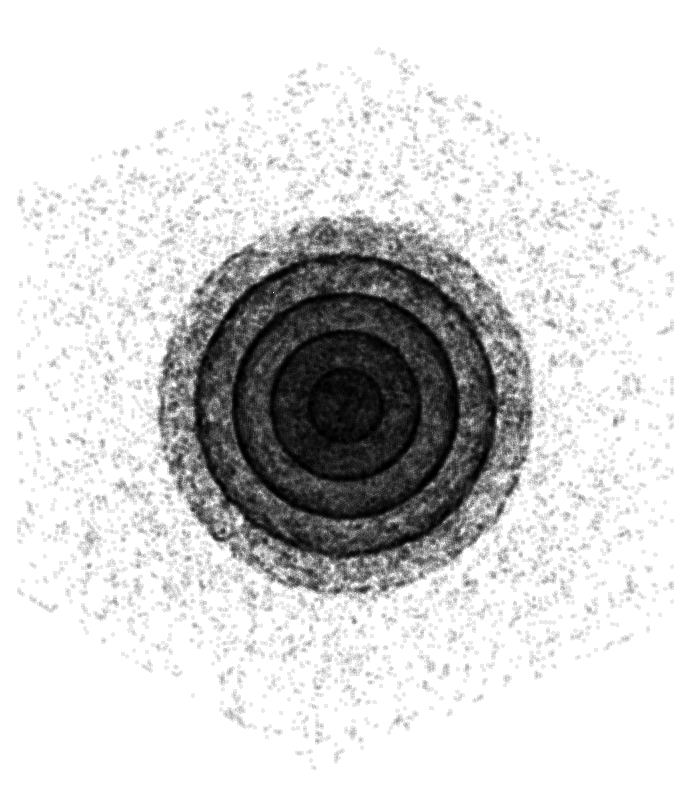
\includegraphics[scale=0.18]{Cannysigma3sphere}&\includegraphics[scale=0.18]{SteerableFilterSigma2sphere}\\
a & b & c \\
\includegraphics[scale=0.18]{stat2dsphere.eps}& \includegraphics[scale=0.18]{T3_sphere}&\includegraphics[scale=0.18]{T13_sphere}\\

d & e & f\\

\end{tabular}
\caption{ Results from a) Canny 2D. b) Canny 3D. c) Steerable. d) 2D Statistical. e) 3D Statistical MR. f) 3D Statistical $\|x\|$.}
\end{figure}
\end{frame}
\subsubsection{Sphere Reversed}
\begin{frame}

\frametitle{Visual Results -Sphere Reversed}
\begin{figure}
\begin{tabular}{c c c }
%\includegraphics[scale=0.2]{SteerableFilterSigma2}&\includegraphics[scale=0.2]{SteerableFilterSigma2rot}&\includegraphics[scale=0.2]{SteerableFilterSigma2sphere}&\includegraphics[scale=0.2]{SteerableFilterSigma2sphereR}\\
\includegraphics[scale=0.18]{canny2dsphereR.eps}&\includegraphics[scale=0.18]{Cannysigma3sphereR}&\includegraphics[scale=0.18]{SteerableFilterSigma2sphereR}\\
a & b & c\\
\includegraphics[scale=0.18]{stat2dsphereR.eps} & \includegraphics[scale=0.18]{T3_sphereR}&\includegraphics[scale=0.18]{T13_sphereR}\\

d & e & f\\
\end{tabular}
\caption{ Results from a) Canny 2D. b) Canny 3D. c) Steerable. d) 2D Statistical. e) 3D Statistical MR. f) 3D Statistical $\|x\|$.}
\end{figure}
\end{frame}
\subsubsection{Multiple Scale}
\begin{frame}[shrink]
\frametitle{Visual Results - Multiple Scale}
\begin{figure}
\begin{tabular}{c c c }
%\includegraphics[scale=0.2]{T3_11}&\includegraphics[scale=0.2]{T3_9}&\includegraphics[scale=0.2]{T3_sphere}&\includegraphics[scale=0.2]{T3_sphereR}\\
\includegraphics[scale=0.2]{canny2dmulti}&\includegraphics[scale=0.2]{Cannysigma3}&\includegraphics[scale=0.2]{SteerableFilterSigma2}\\
a & b & c \\
\includegraphics[scale=0.2]{stat2dmulti.eps}&\includegraphics[scale=0.2]{T3_11}&\includegraphics[scale=0.2]{T13_9}\\
d & e & f\\

\end{tabular}
\caption{ Results from a) Canny 2D. b) Canny 3D. c) Steerable. d) 2D Statistical. e) 3D Statistical MR. f) 3D Statistical $\|x\|$.}
\end{figure}
\end{frame}
\subsubsection{Multiple Scale Rotated}
\begin{frame}
\frametitle{Visual Results - Multiple Scale Rotated}
\begin{figure}
\begin{tabular}{c c  c }
%\includegraphics[scale=0.2]{T13_9}&\includegraphics[scale=0.2]{T13_9rot}&\includegraphics[scale=0.2]{T13_sphere}&\includegraphics[scale=0.2]{T13_sphereR}\\
\includegraphics[scale=0.2]{canny2dmultiR}&\includegraphics[scale=0.2]{Cannysigma3rot}&\includegraphics[scale=0.2]{SteerableFilterSigma2rot}\\
a & b & c \\
\includegraphics[scale=0.2]{stat2dmultiR.eps}&\includegraphics[scale=0.2]{T3_9}&\includegraphics[scale=0.2]{T13_9rot}\\
d & e & f\\

\end{tabular}
\caption{ Results from a) Canny 2D. b) Canny 3D. c) Steerable. d) 2D Statistical. e) 3D Statistical MR. f) 3D Statistical $\|x\|$.}
\end{figure}
\end{frame}
\subsection{MRI Results}
\begin{frame}
\frametitle{Real Image Results}
\begin{figure}
\begin{tabular}{c c c}
\includegraphics[scale=0.25]{headsteer}&\includegraphics[scale=0.25]{headcanny}&\includegraphics[scale=0.25]{headT}\\
Steerable & Canny & Statistical

\end{tabular}
\end{figure}
\end{frame}
\section{Conclusions}
\subsection{Conclusions}
\begin{frame}
\frametitle{Conclusions}
\begin{itemize}
\item Outperforms 3D Canny and Steerable filters, improved response to texture and noise.
\item Outperforms all 2D edge detection methods.
\item When possible, 3D surface detection should always be used instead of 2D, and where texture defines image boundaries, Statistical methods should be employed.
\end{itemize}
 
\end{frame}
\subsection{Future Work}
\begin{frame}
\frametitle{ Future Work }
\begin{itemize}
\item Synthetic data creation.
\item Statistical tests
\item Mask shape
\item Real World application testing. (Active Contours/surfaces, snakes GVFCs, etc) 
\end{itemize}
\end{frame}
\subsection{End}
		\begin{frame}
				\begin{center}
				\textbf{End}\\
		
				{\Huge{pub ?}}
				\end{center}
			


	\end{frame}


%------------------------------------------------	
	
	\end{document}
